%-*- coding: utf-8 -*-
\documentclass{beamer}

\usepackage[frenchb]{babel}
\usepackage[T1]{fontenc}
\usepackage[utf8]{inputenc}
\graphicspath{{images/}}
\usepackage{csquotes}

\usetheme{Warsaw}

\title{Projet Vitameal}
\subtitle{Restauration en milieu hospitalier}
\author{Nicolas Symphorien, Sonia Othmani, Jean-Félix Benitez}
\institute{CNAM}
\date{06/07/2017}

\logo{
\includegraphics[height=10mm]{ipst-cnam.png}}
\setbeamertemplate{background canvas}{
\includegraphics[width=\paperwidth,height=\paperheight]{fond_200.png}} % Width pour la largeur, height pour la hauteur de l'image

\begin{document}
\begin{frame}[plain]
  \titlepage
\end{frame}

\begin{frame}
  \frametitle{Sommaire}
  \tableofcontents
\end{frame}

\section{Définition du problème}
\begin{frame}[label=definitionDuProbleme]
\frametitle{Définition du problème}
L'élaboration de menus dans un hôpital pour la restauration des patients
est une tâche complexe, et doit tenir compte des différentes pathologies
rencontrées. Faute de moyens (temps et argent) seules quelques grandes
lignes de restauration sont retenues; alors qu'idéalement, chaque
patient devrait pourvoir avoir un repas adapté à sa pathologie.
\end{frame}

\subsection{Solution envisagée}
\begin{frame}[label=solutionEnvisagée]
\frametitle{Solution envisagée}
Le projet Vitameal a pour objectif de faire correspondre au mieux la planification des régimes et des
prescriptions diététiques aux repas réellement servis au patient. Il consiste en un outil interfaçant la
gestion de production, la prise de commande et le suivi nutritionnel des repas.
\end{frame}

\subsection{Périmètre}
\begin{frame}[label=perimetre]
\frametitle{Périmètre}
C'est un diététicien qui renseigne le profil diététique des patients,
sous les directives des médecins. C'est aussi un diététicien qui élabore
les menus des patients. L'outil élaborera donc
les menus par filtrage des produits correspondants aux profils
diététiques des patients. Pour des raisons de simplifications, nous nous limiterons dans ce projet aux seuls patients adolescents et adultes, à l'exclusion des personnes agées.
\end{frame}

\section{Analyse des exigences}
\subsection{Analyse}
\begin{frame}[label=analyseDesExigences] %allowframebreaks
\frametitle{Analyse des exigences}
\begin{itemize}
  \item Partie prenantes
  \begin{itemize}
    \item Participantes~: les diététiciens, le service restauration
    \item Concernés~: les médecins, la direction (budget)
    \item Impactées~: les patients
  \end{itemize}
  \item Les besoins
  \begin{itemize}
    \item Les diététiciens renseignent les profils diététiques de chaque patient.
    \item Les diététiciens lance l'élaboration automatique des menus.
    \item Le service restauration commande les produits et ingrédients mis en œuvre dans les menus
    \item Le service restauration prépare les menus élaborés.
  \end{itemize}
  \item Les contraintes
  \begin{itemize}
    \item Les médecins doivent pouvoir vérifier / valider les profils diététiques des patients.
    \item La direction fixe un budget maximum par menu.
  \end{itemize}
\end{itemize}
\end{frame}

\subsection{Exigences}
\begin{frame}
 \frametitle{Exigences}
Chaque exigence est composée de 11 champs:
\begin{itemize}
\item \textbf{numéro:} Formé comme suit REQ\_12345
\item \textbf{Titre:} Titre ou description courte
\item \textbf{Corps:} Expression de l'exigence
\item \textbf{Type:} Utilisateur, Métier, Système, Contrainte
\item \textbf{Nature:} Fonctionnelle, Ergonomie, Robustesse, Performance, Sécurité
\item \textbf{Origine:} D'où vient une exigence ?
\item \textbf{Version:} ou niveau de maturité, Initiale, Intermédiaire, Finale
\item \textbf{Priorité:} MoSCoW, Must, Should, Could, Won't
\item \textbf{Validée:} L'exigences a-t-elle été validée ? (Oui / Non)
\item \textbf{Liens:} Liens
\item \textbf{Test:} Définition du test qui validera l'exigence.
\end{itemize}

\url{../Exigences/Exigences.html}
\end{frame}

\section{Cas d'Utilisations}

\begin{frame}
\frametitle{Cas d'Utilisations}
\begin{figure}[H]
\label{schema}
  \centering
      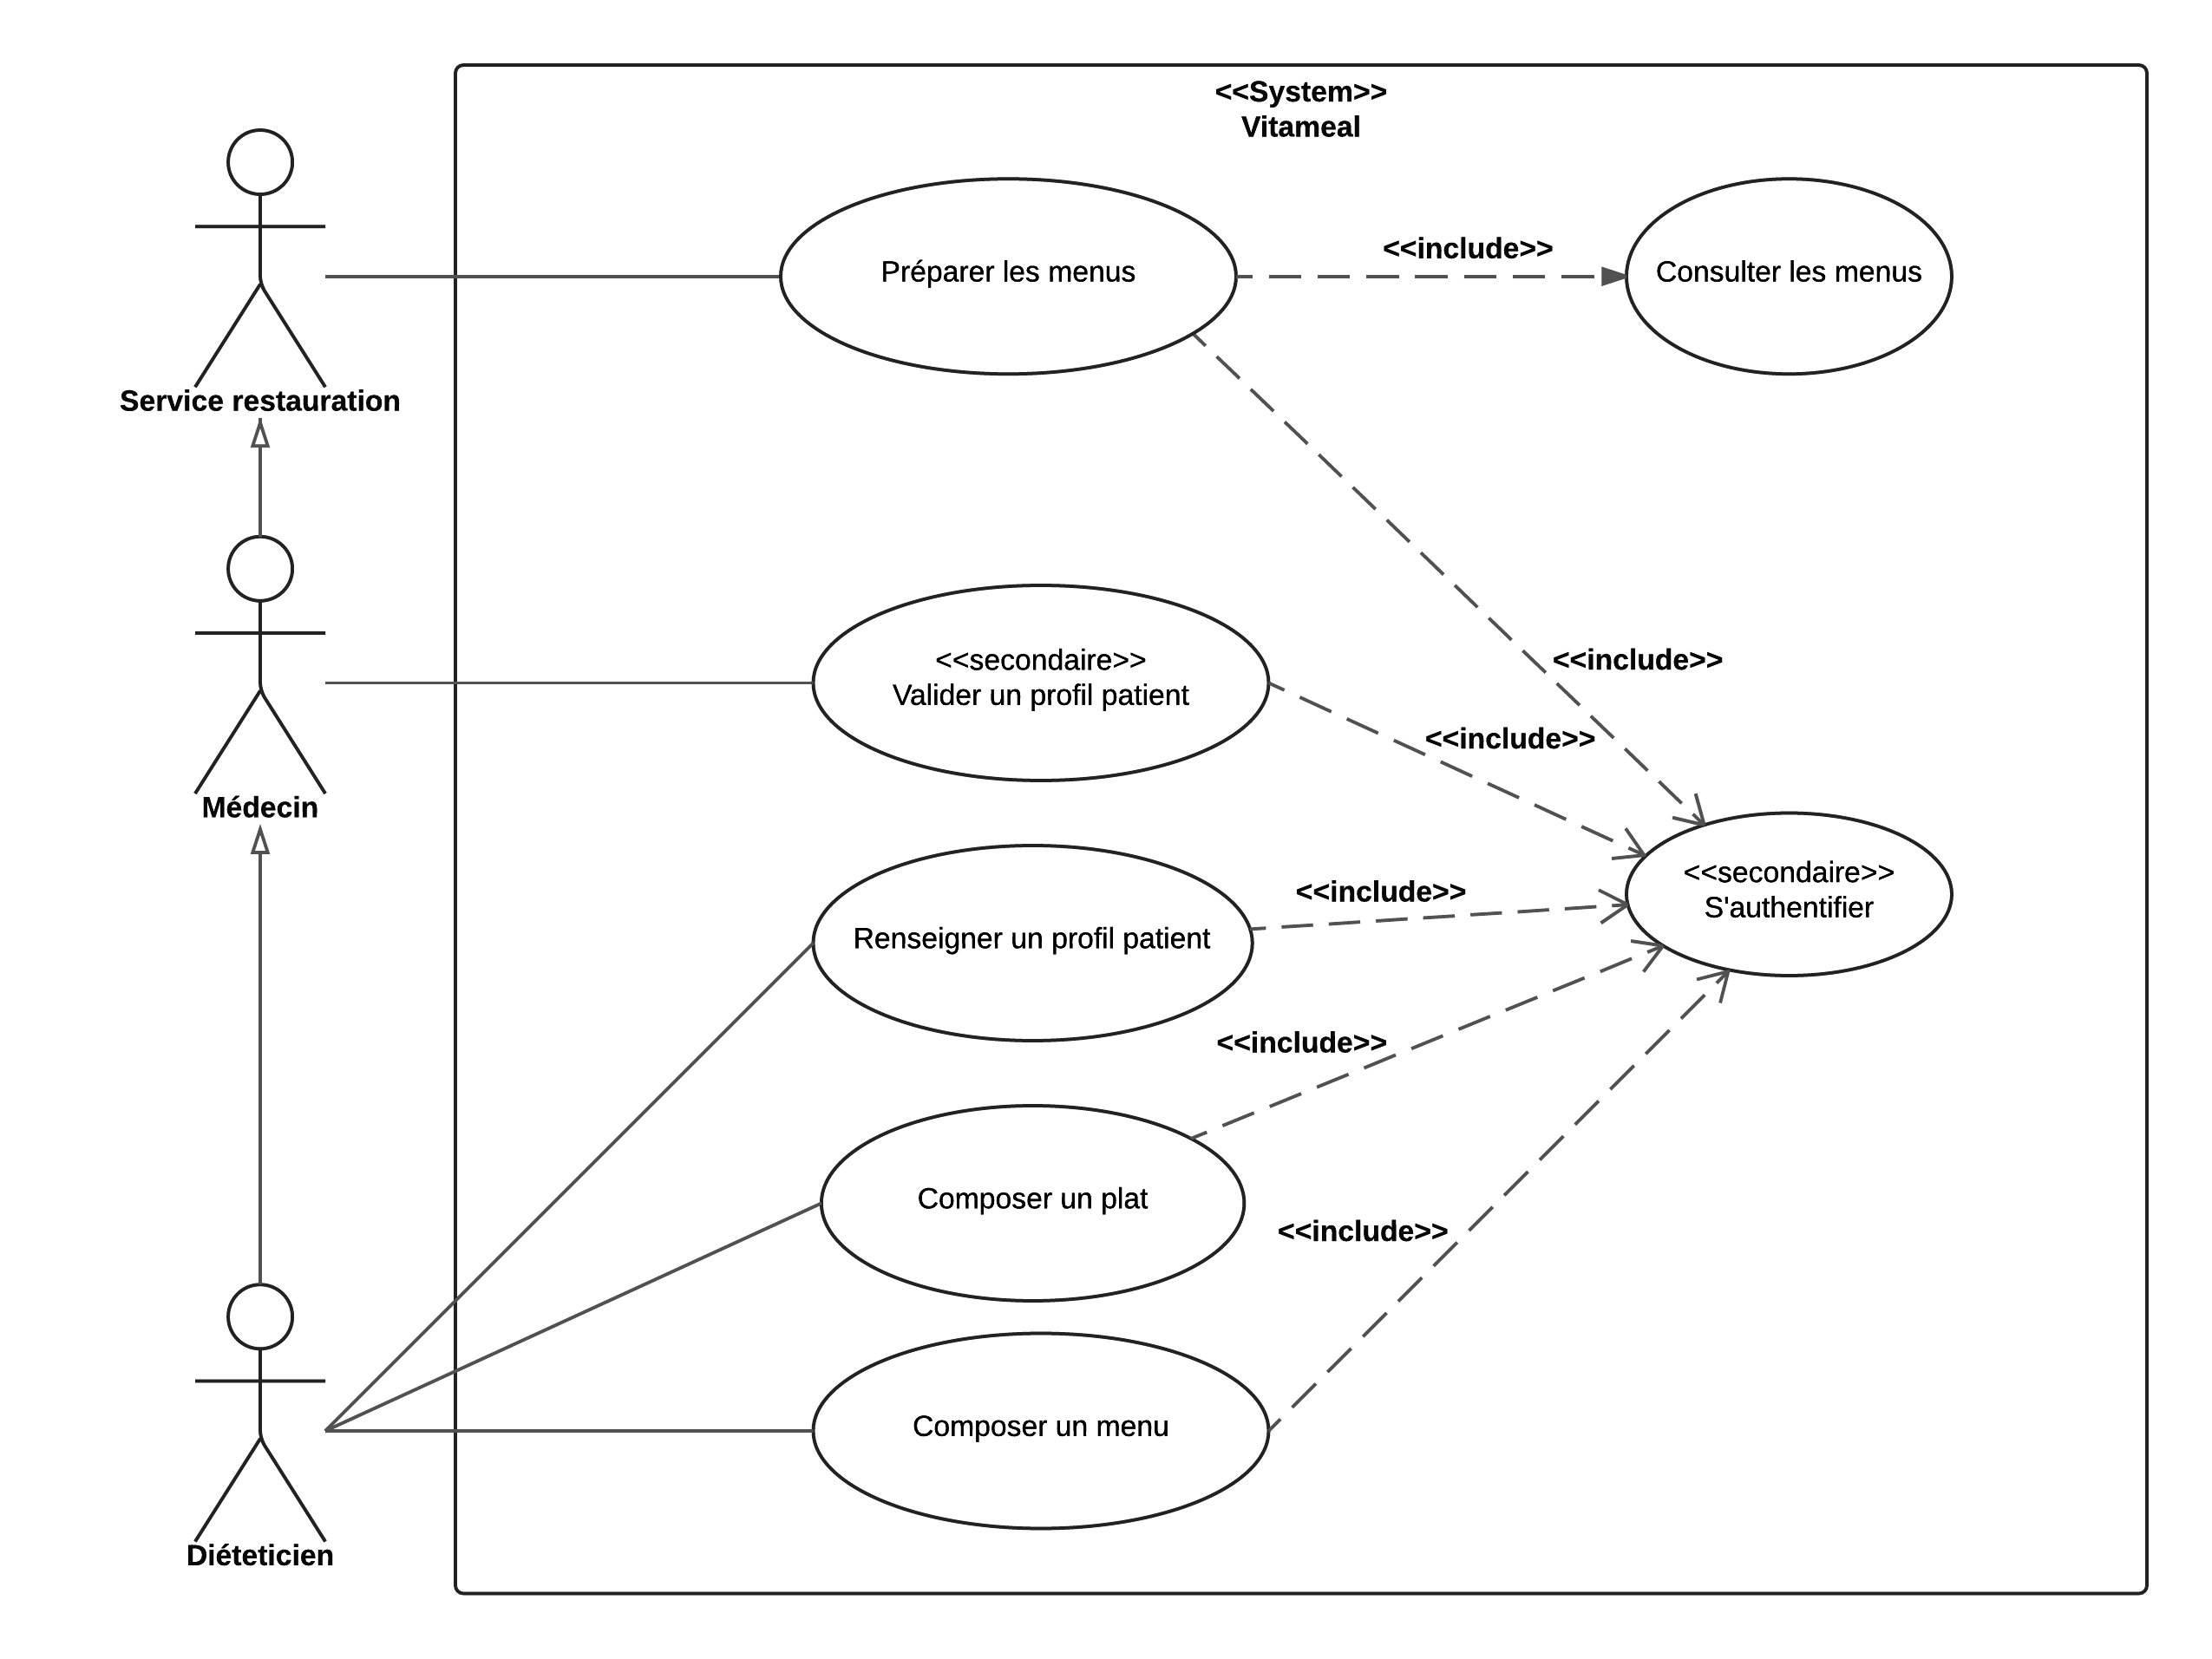
\includegraphics[scale=0.4]{../CasDUtilisations/diagramme_cas_utilisation.png}
\end{figure}
\end{frame}

\subsection{Profil patient}
\begin{frame}[plain]{}
%\frametitle{Profil patient}
%%-*- coding: utf-8 -*-
\subsection{Renseigner les profils patients}

\begin{figure}[!h]
  \label{diagramme-renseigner-les-profils-patients}
  \centering
  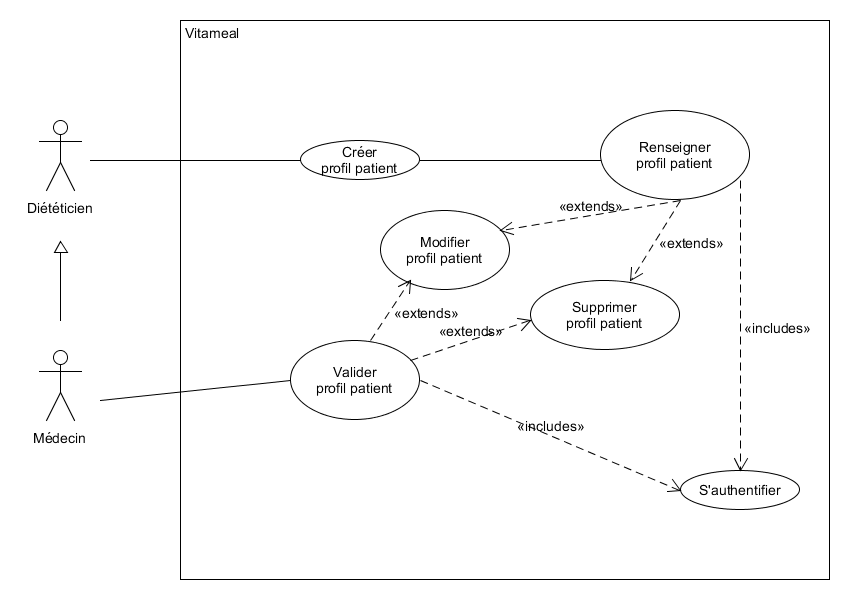
\includegraphics[width=0.9\textwidth]{../../CasDUtilisations/ProfilPatient/ProfilPatient.png}
  \caption{Use case renseigner les profils patients}
\end{figure}

\subsubsection{UC400 - Renseigner profil patient}
\begin{description}
\item [Nom :] Renseigner profil patient
\item [ID :] UC400
\item [Description :] Le diététicien souhaite pouvoir renseigner un profil patient.
\item [Auteur :] Sonia OTHMANI
\item [Date :] 08/05/2017
\item [Acteurs :] Le diététicien
\item [Pré-condition :] L’utilisateur doit être identifié en tant que diététicien (Voir cas d’utilisation \enquote{S’authentifier})
\item [Scénario principal :]
  \begin{enumerate}
  \item Le système affiche une page permettant de créer un profil patient.
  \item L’utilisateur complète les champs relatifs au patient : nom, prénom, date de naissance, pathologies, allergies, régime alimentaire prescrit.
  \item L’utilisateur valide le profil patient.
  \item Le système enregistre le profil patient.
  \end{enumerate}
\item [Scénario alternatif :] Aucun
\item [Post-Conditions :] Le profil patient est créé et enregistré.
\end{description}

\subsubsection{UC401 - Modifier profil patient}
\begin{description}
\item [Nom :] Modifier profil patient
\item [ID :] UC401
\item [Description :] Le diététicien souhaite pouvoir modifier un profil patient.
\item [Auteur :] Sonia OTHMANI
\item [Date :] 08/05/2017
\item [Acteurs :] Le diététicien
\item [Pré-condition :] L’utilisateur doit être identifié en tant que diététicien (Voir cas d’utilisation \enquote{S’authentifier})
\item [Scénario principal :]
  \begin{enumerate}
  \item Le système affiche une liste de profils patients.
  \item L’utilisateur sélectionne la fiche patient à modifier.
  \item L’utilisateur modifie le profil patient.
  \item L’utilisateur valide le profil patient.
  \item Le système enregistre le profil patient modifié.
  \end{enumerate}
\item [Scénario alternatif :] Aucun
\item [Post-Conditions :] Le profil patient est modifié et enregistré.
\end{description}

\subsubsection{UC402 - Supprimer profil patient}
\begin{description}
\item [Nom :] Supprimer profil patient
\item [ID :] UC402
\item [Description :] Le diététicien souhaite pouvoir supprimer un profil patient.
\item [Auteur :] Sonia OTHMANI
\item [Date :] 08/05/2017
\item [Acteurs :] Le diététicien
\item [Pré-condition :] L’utilisateur doit être identifié en tant que diététicien (Voir cas d’utilisation \enquote{S’authentifier})
\item [Scénario principal :]
  \begin{enumerate}
  \item Le système affiche une liste de profils patients.
  \item L’utilisateur sélectionne la fiche patient à supprimer .
  \item L’utilisateur supprime le profil patient.
  \item Le système enregistre la suppression.
  \end{enumerate}
\item [Scénario alternatif :] Aucun
\item [Post-Conditions :] Le profil patient est supprimé
\end{description}

\begin{figure}
\centering
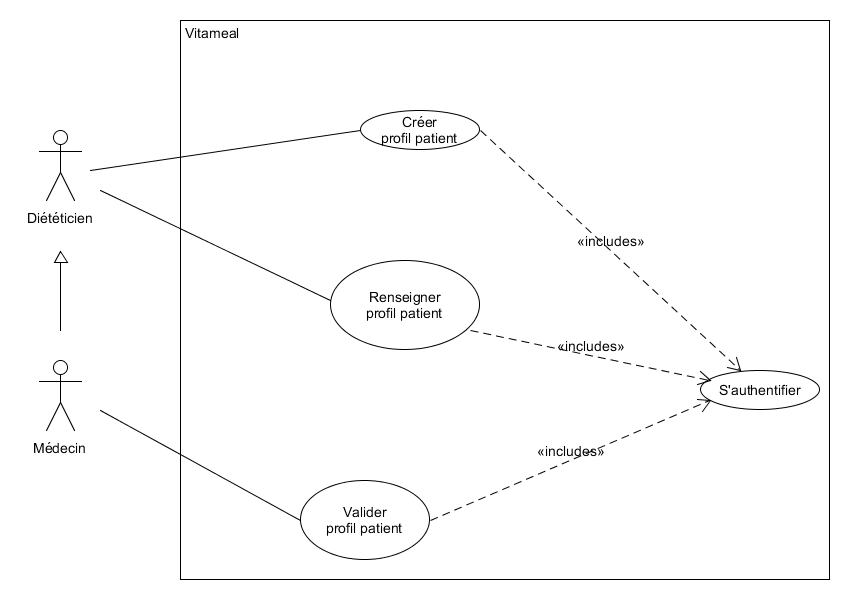
\includegraphics[scale=0.4]{../CasDUtilisations/ProfilPatient/UseCaseProfilPatient.png}
\end{figure}
\end{frame}

\begin{frame}[plain]{}
\begin{figure}
\centering
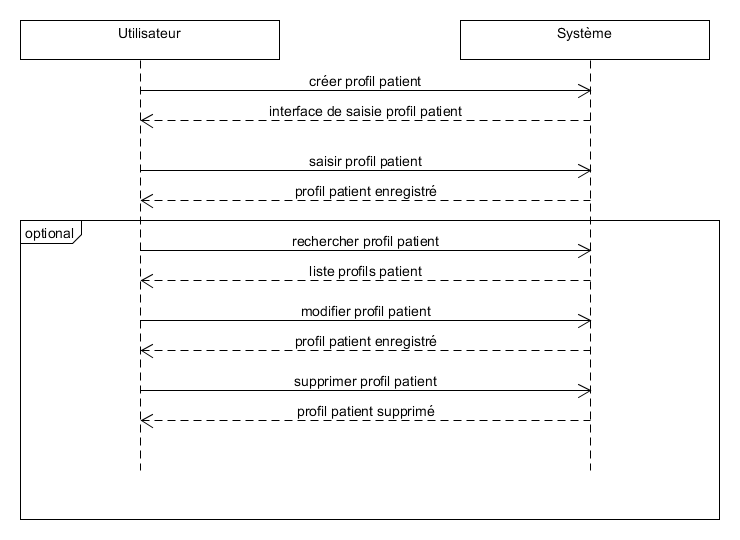
\includegraphics[scale=0.4]{../CasDUtilisations/ProfilPatient/diagseqProfilPatient.png}
\end{figure}
\end{frame}

\begin{frame}[plain]{}
\begin{figure}
\centering
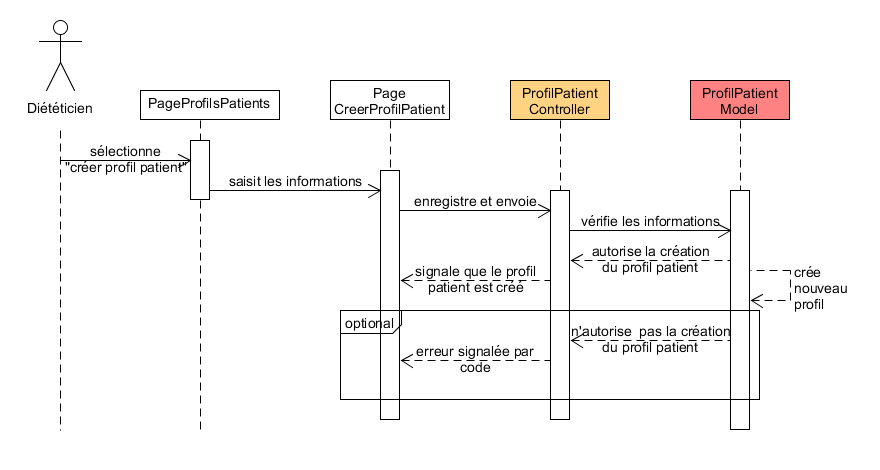
\includegraphics[scale=0.4]{../CasDUtilisations/ProfilPatient/diagSrqDetaillProfilPatient.png}
\end{figure}
\end{frame}

\begin{frame}[plain]{}
\begin{figure}
\centering
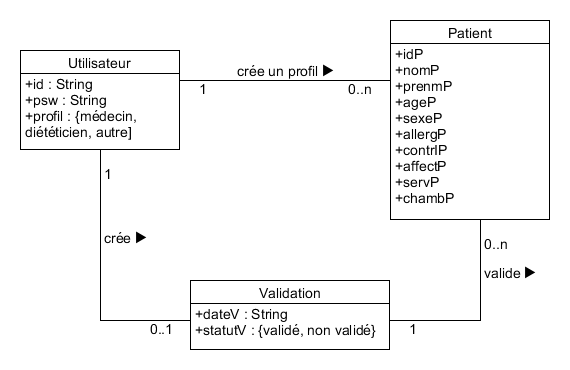
\includegraphics[scale=0.5]{../CasDUtilisations/ProfilPatient/diagclassProfilPatient.png}
\end{figure}
\end{frame}

\subsection{Composer un plat}

\begin{frame}[plain]{}
\begin{figure}
\centering
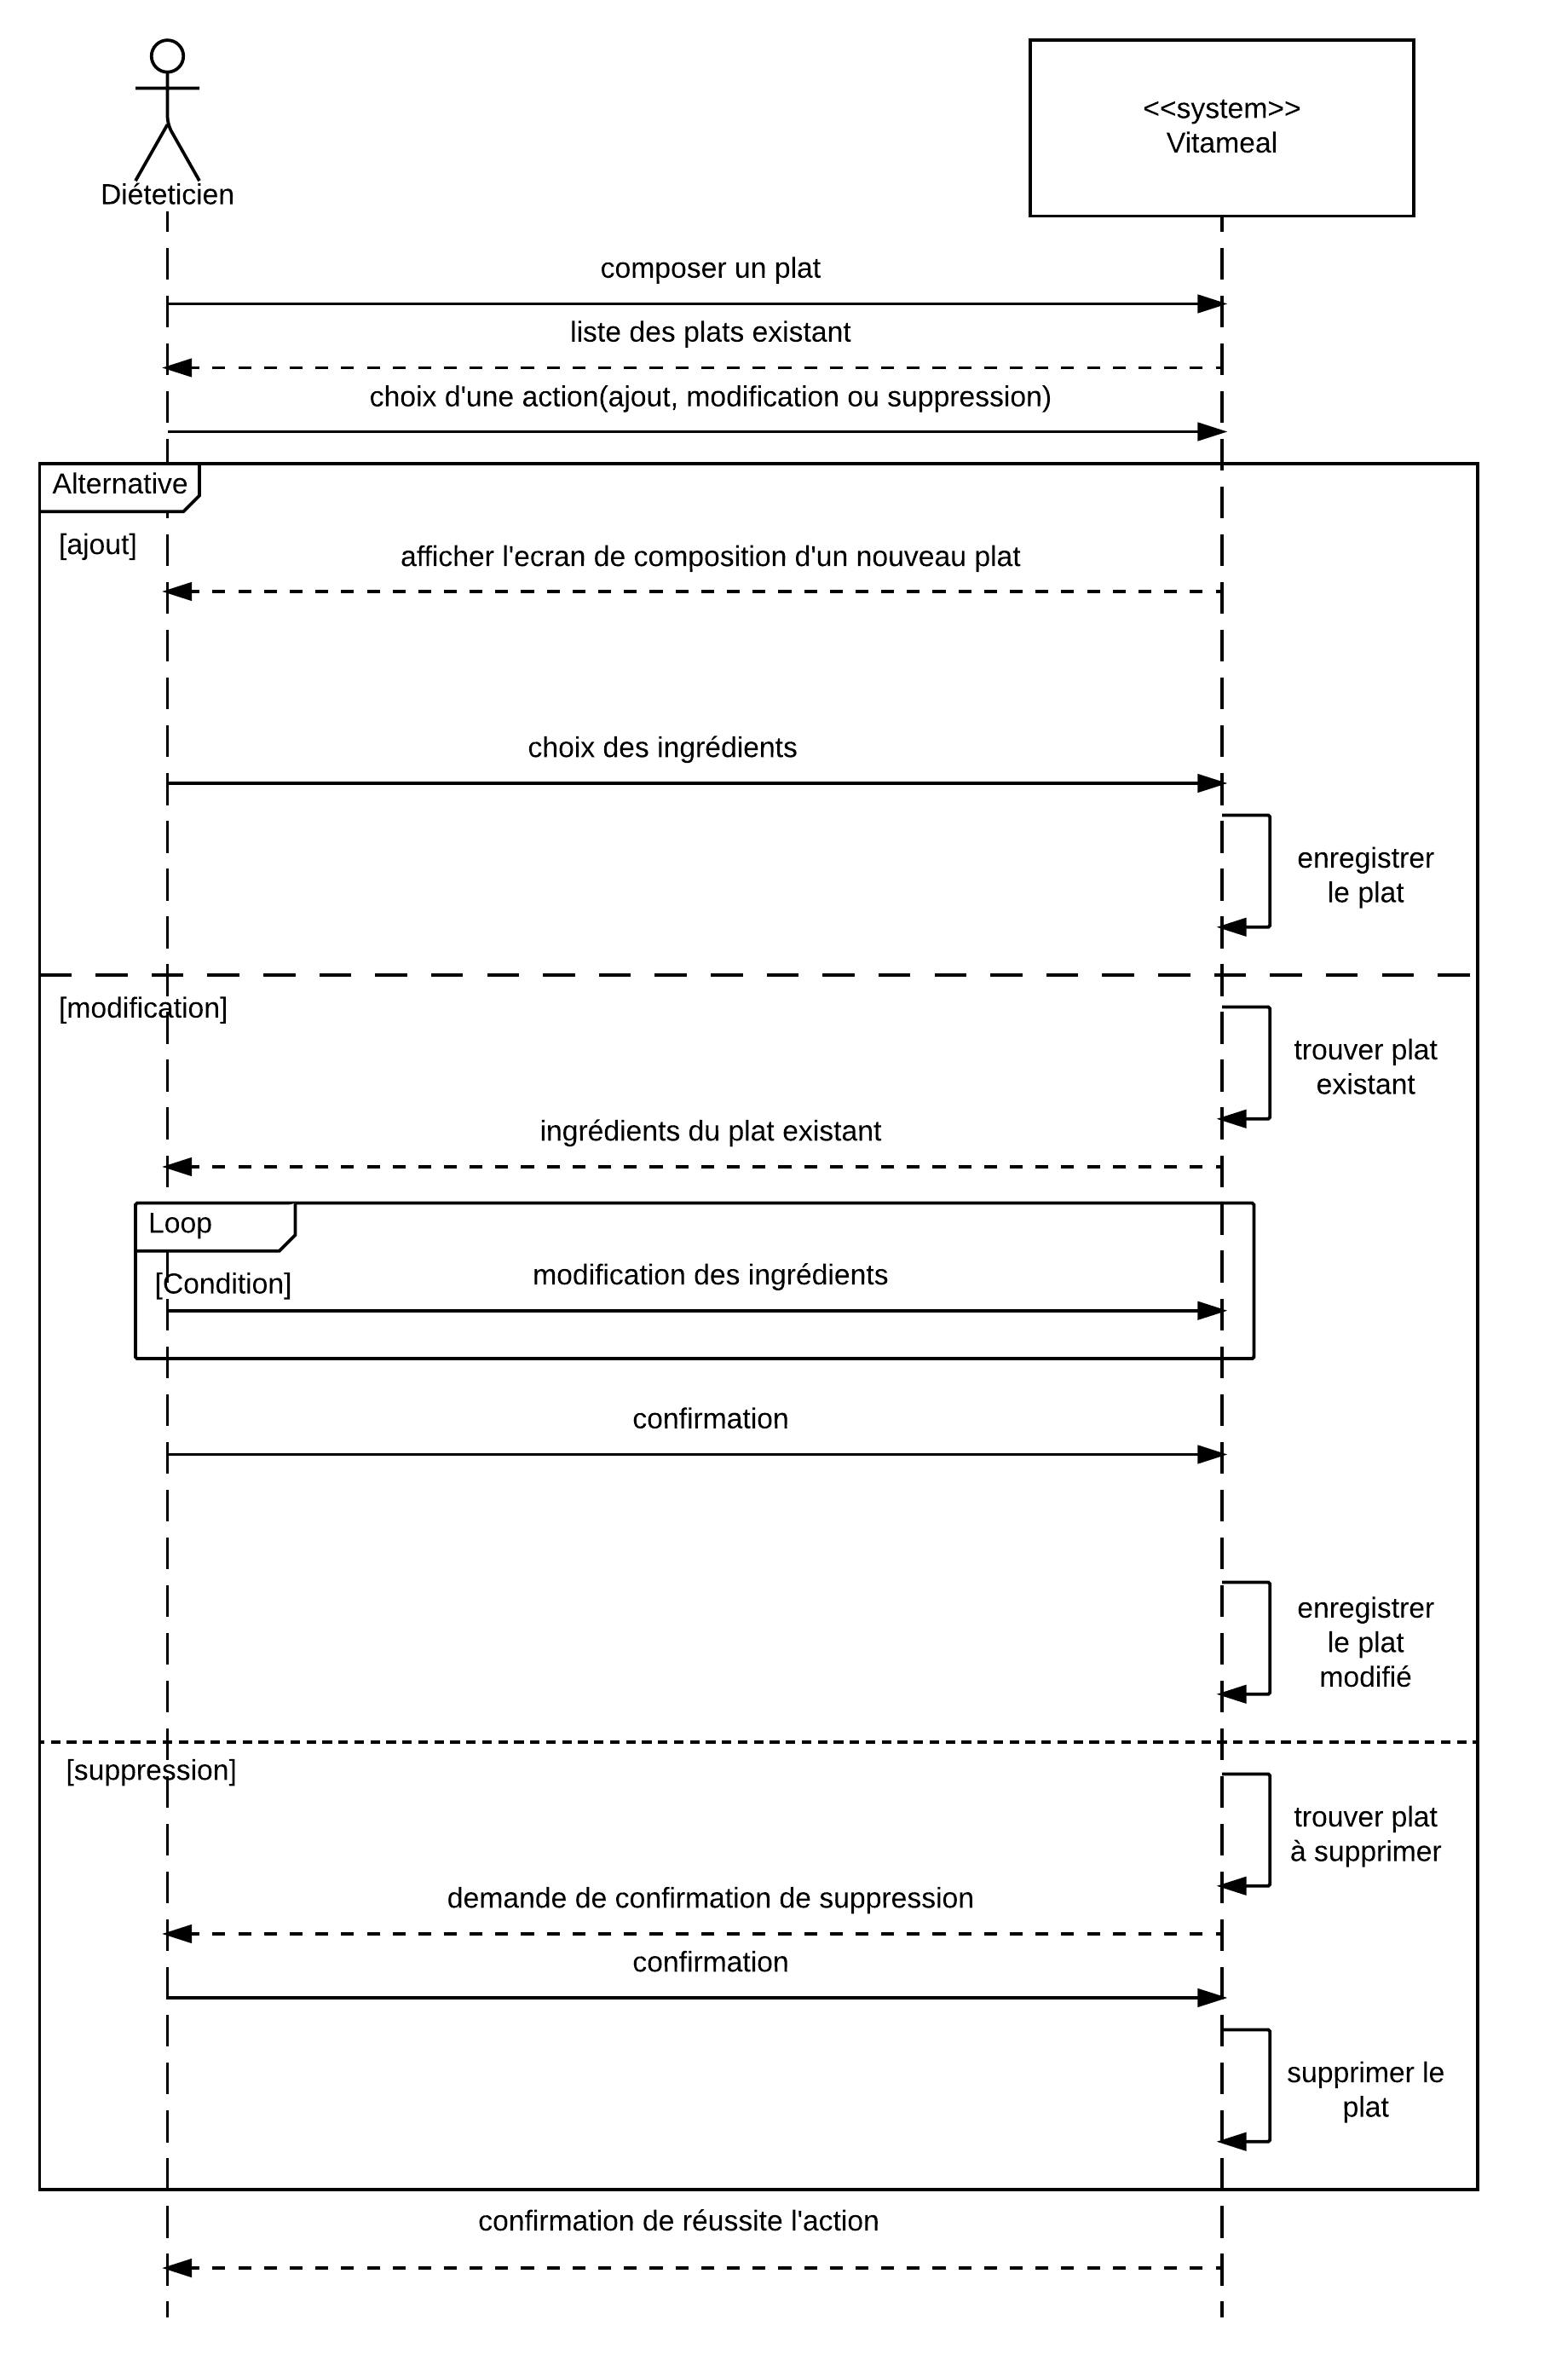
\includegraphics[scale=0.125]{../CasDUtilisations/CompositionPlat/sequence_UC_ComposerPlat.png}
\end{figure}
\end{frame}

\begin{frame}[plain]{}
\begin{figure}
\centering
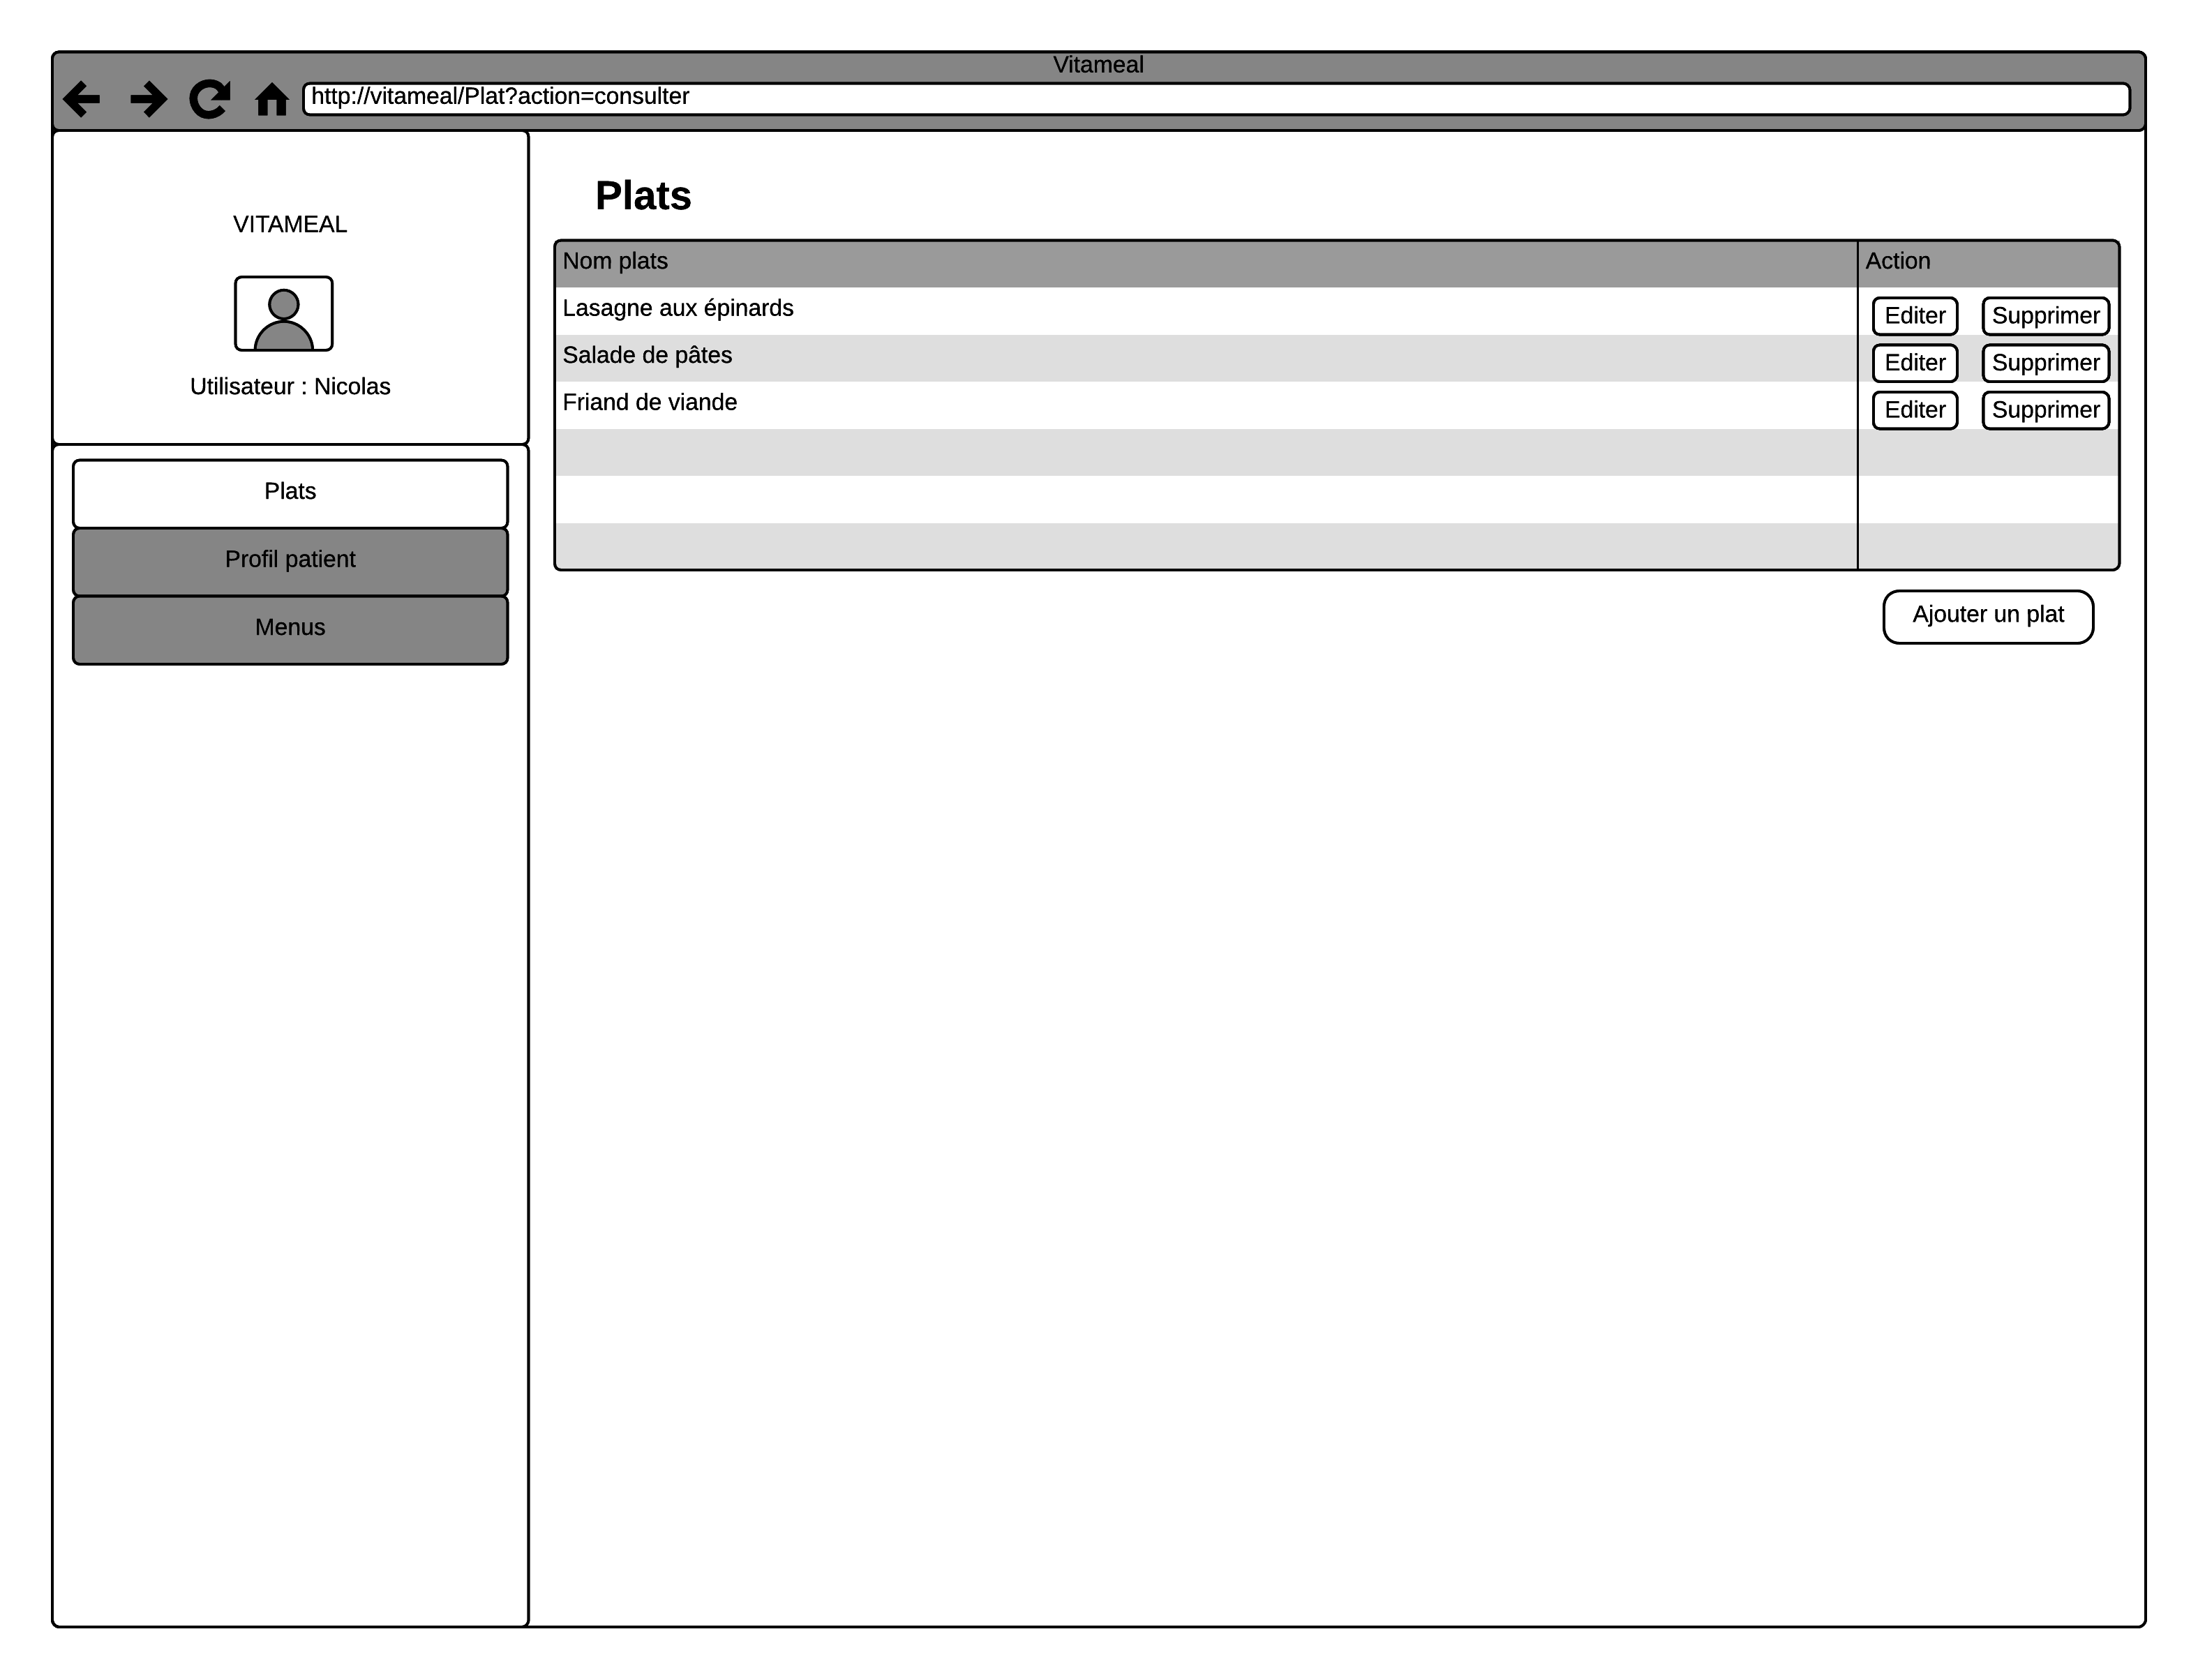
\includegraphics[scale=0.4]{../CasDUtilisations/CompositionPlat/maquette_EcranConsulterPlats.png}
\caption{Maquette de consultation d'un plat}
\label{MaquetteConsultationPlat}
\end{figure}
\end{frame}

\begin{frame}[plain]{}
\begin{figure}
\centering
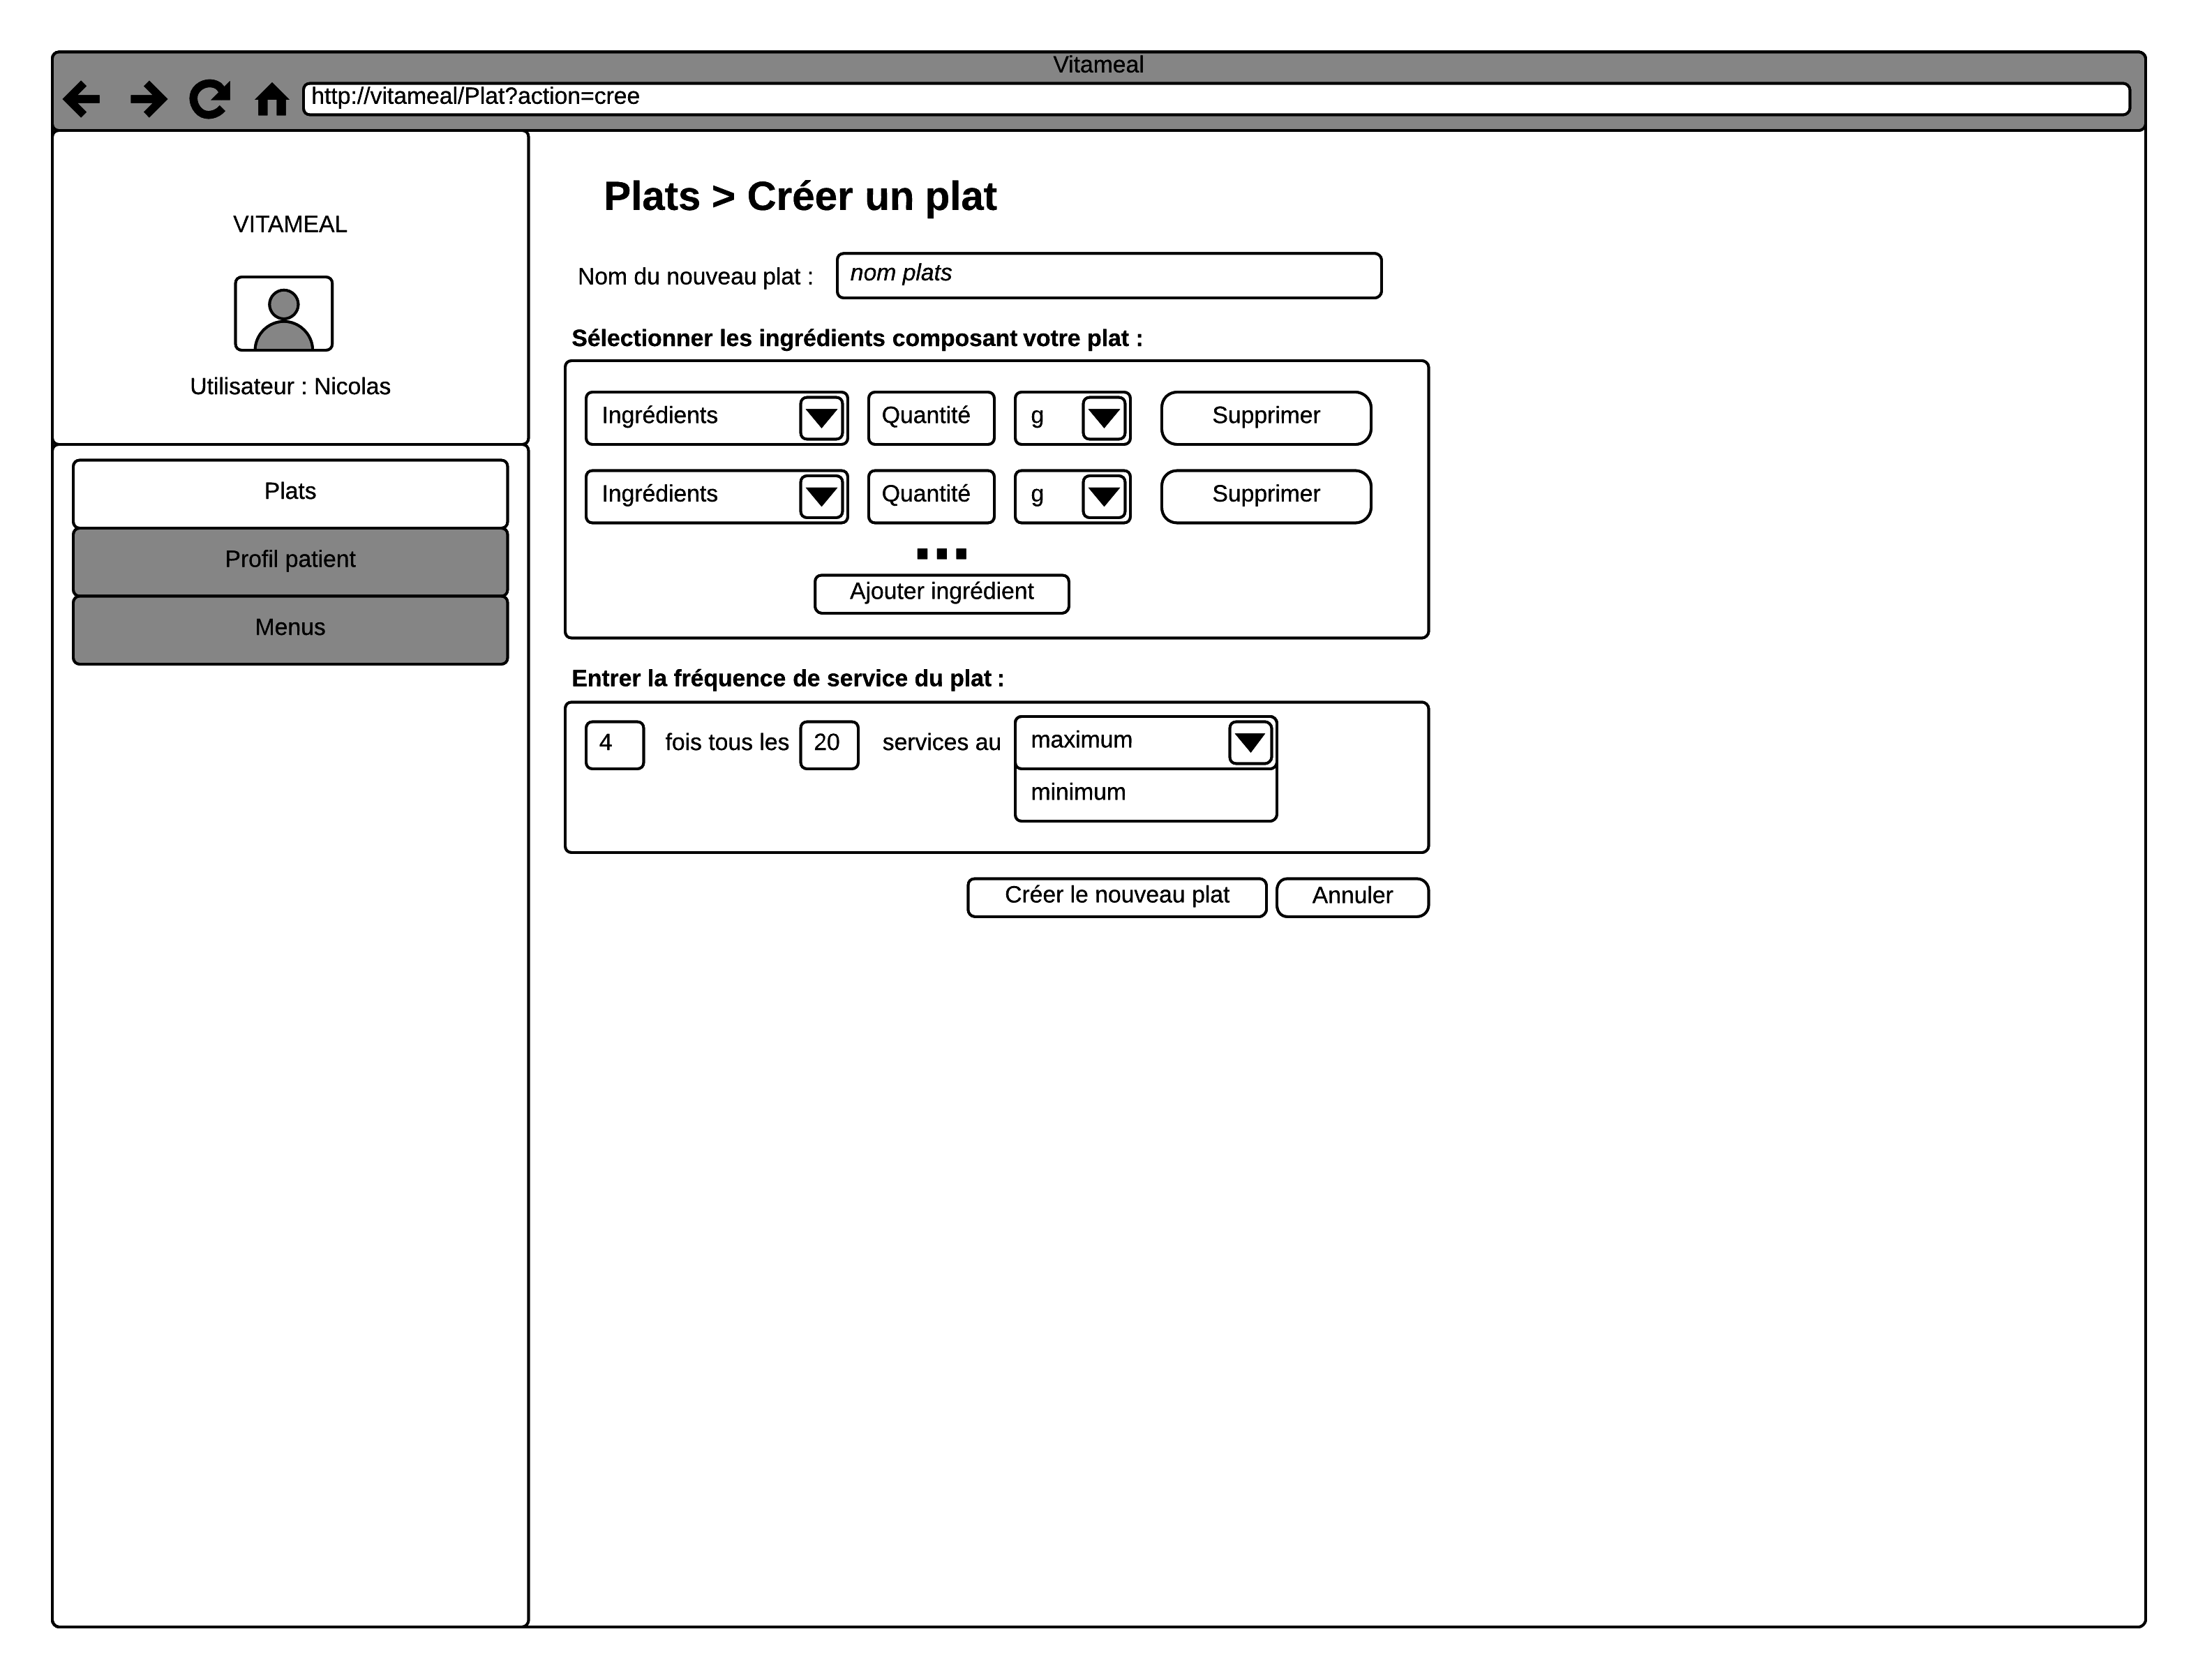
\includegraphics[scale=0.4]{../CasDUtilisations/CompositionPlat/maquette_EcranCreationPlat.png}
\caption{Maquette de la création d'un plat}
\label{MaquetteCreationPlat}
\end{figure}
\end{frame}

\begin{frame}[plain]{}
\begin{figure}
\centering
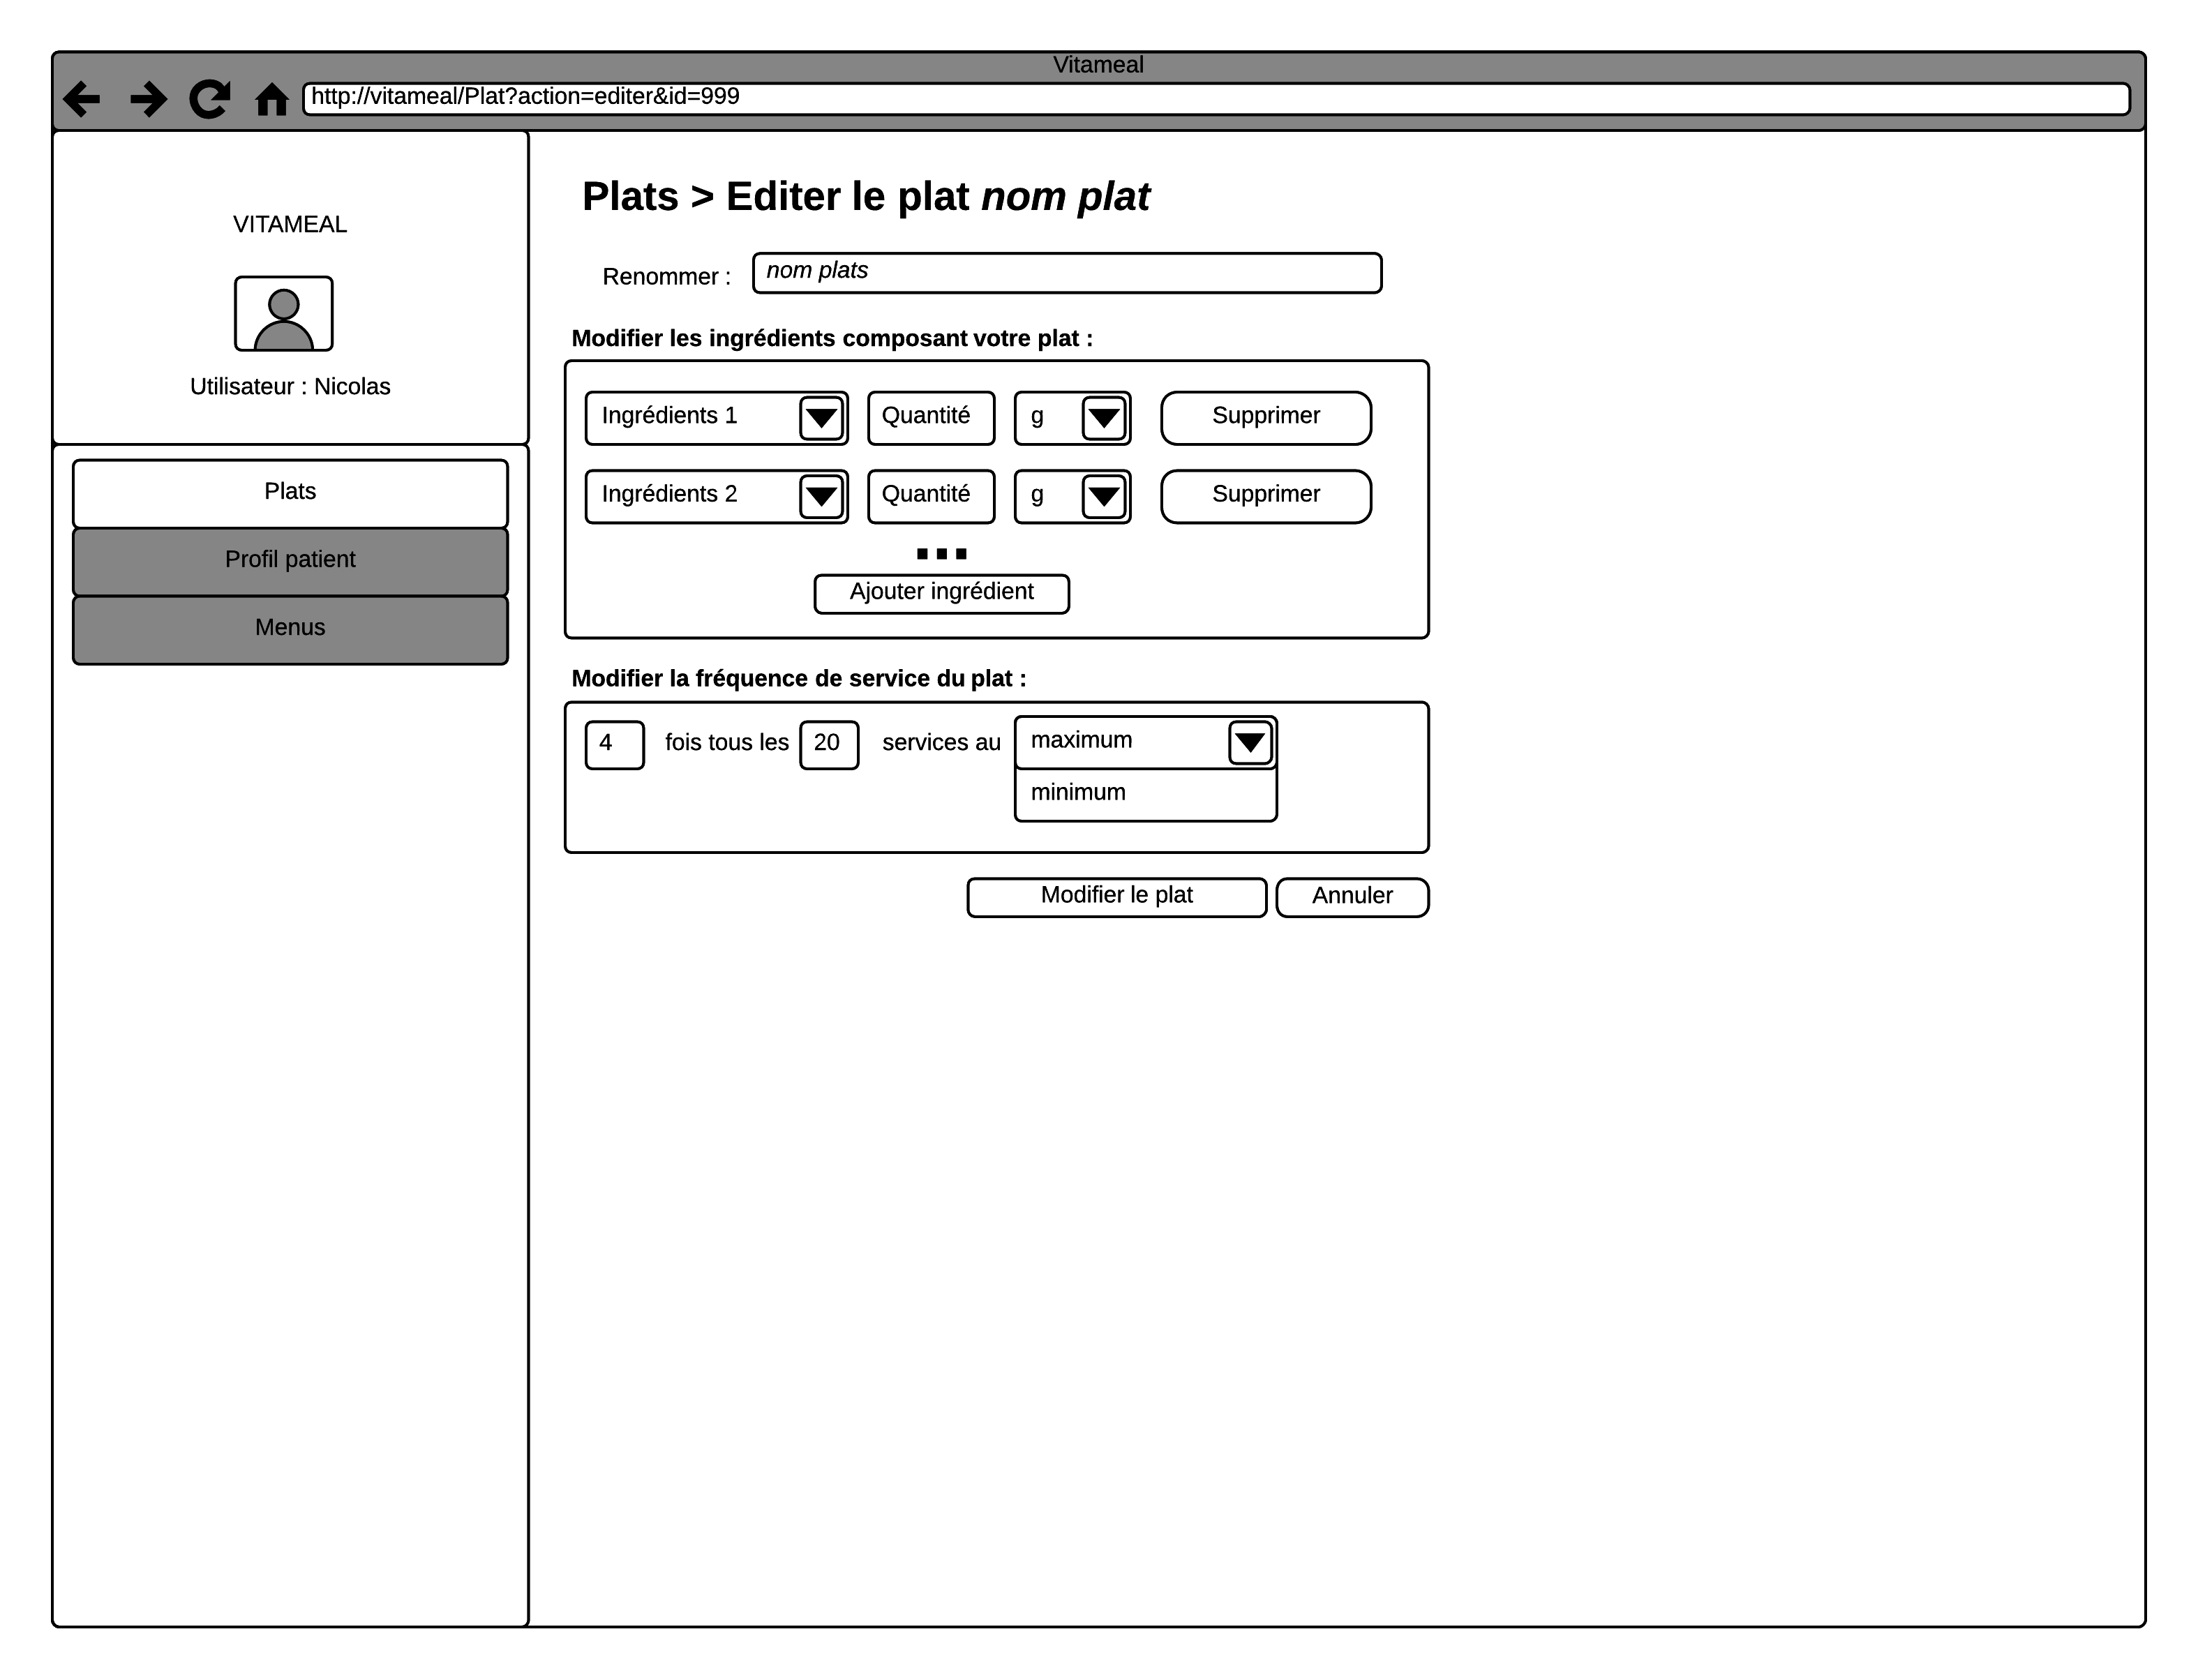
\includegraphics[scale=0.4]{../CasDUtilisations/CompositionPlat/maquette_EcranEditionPlat.png}
\caption{Maquette de l'édition d'un plat}
\label{MaquetteEditionPlat}
\end{figure}
\end{frame}

\begin{frame}[plain]{}
\begin{figure}
\centering
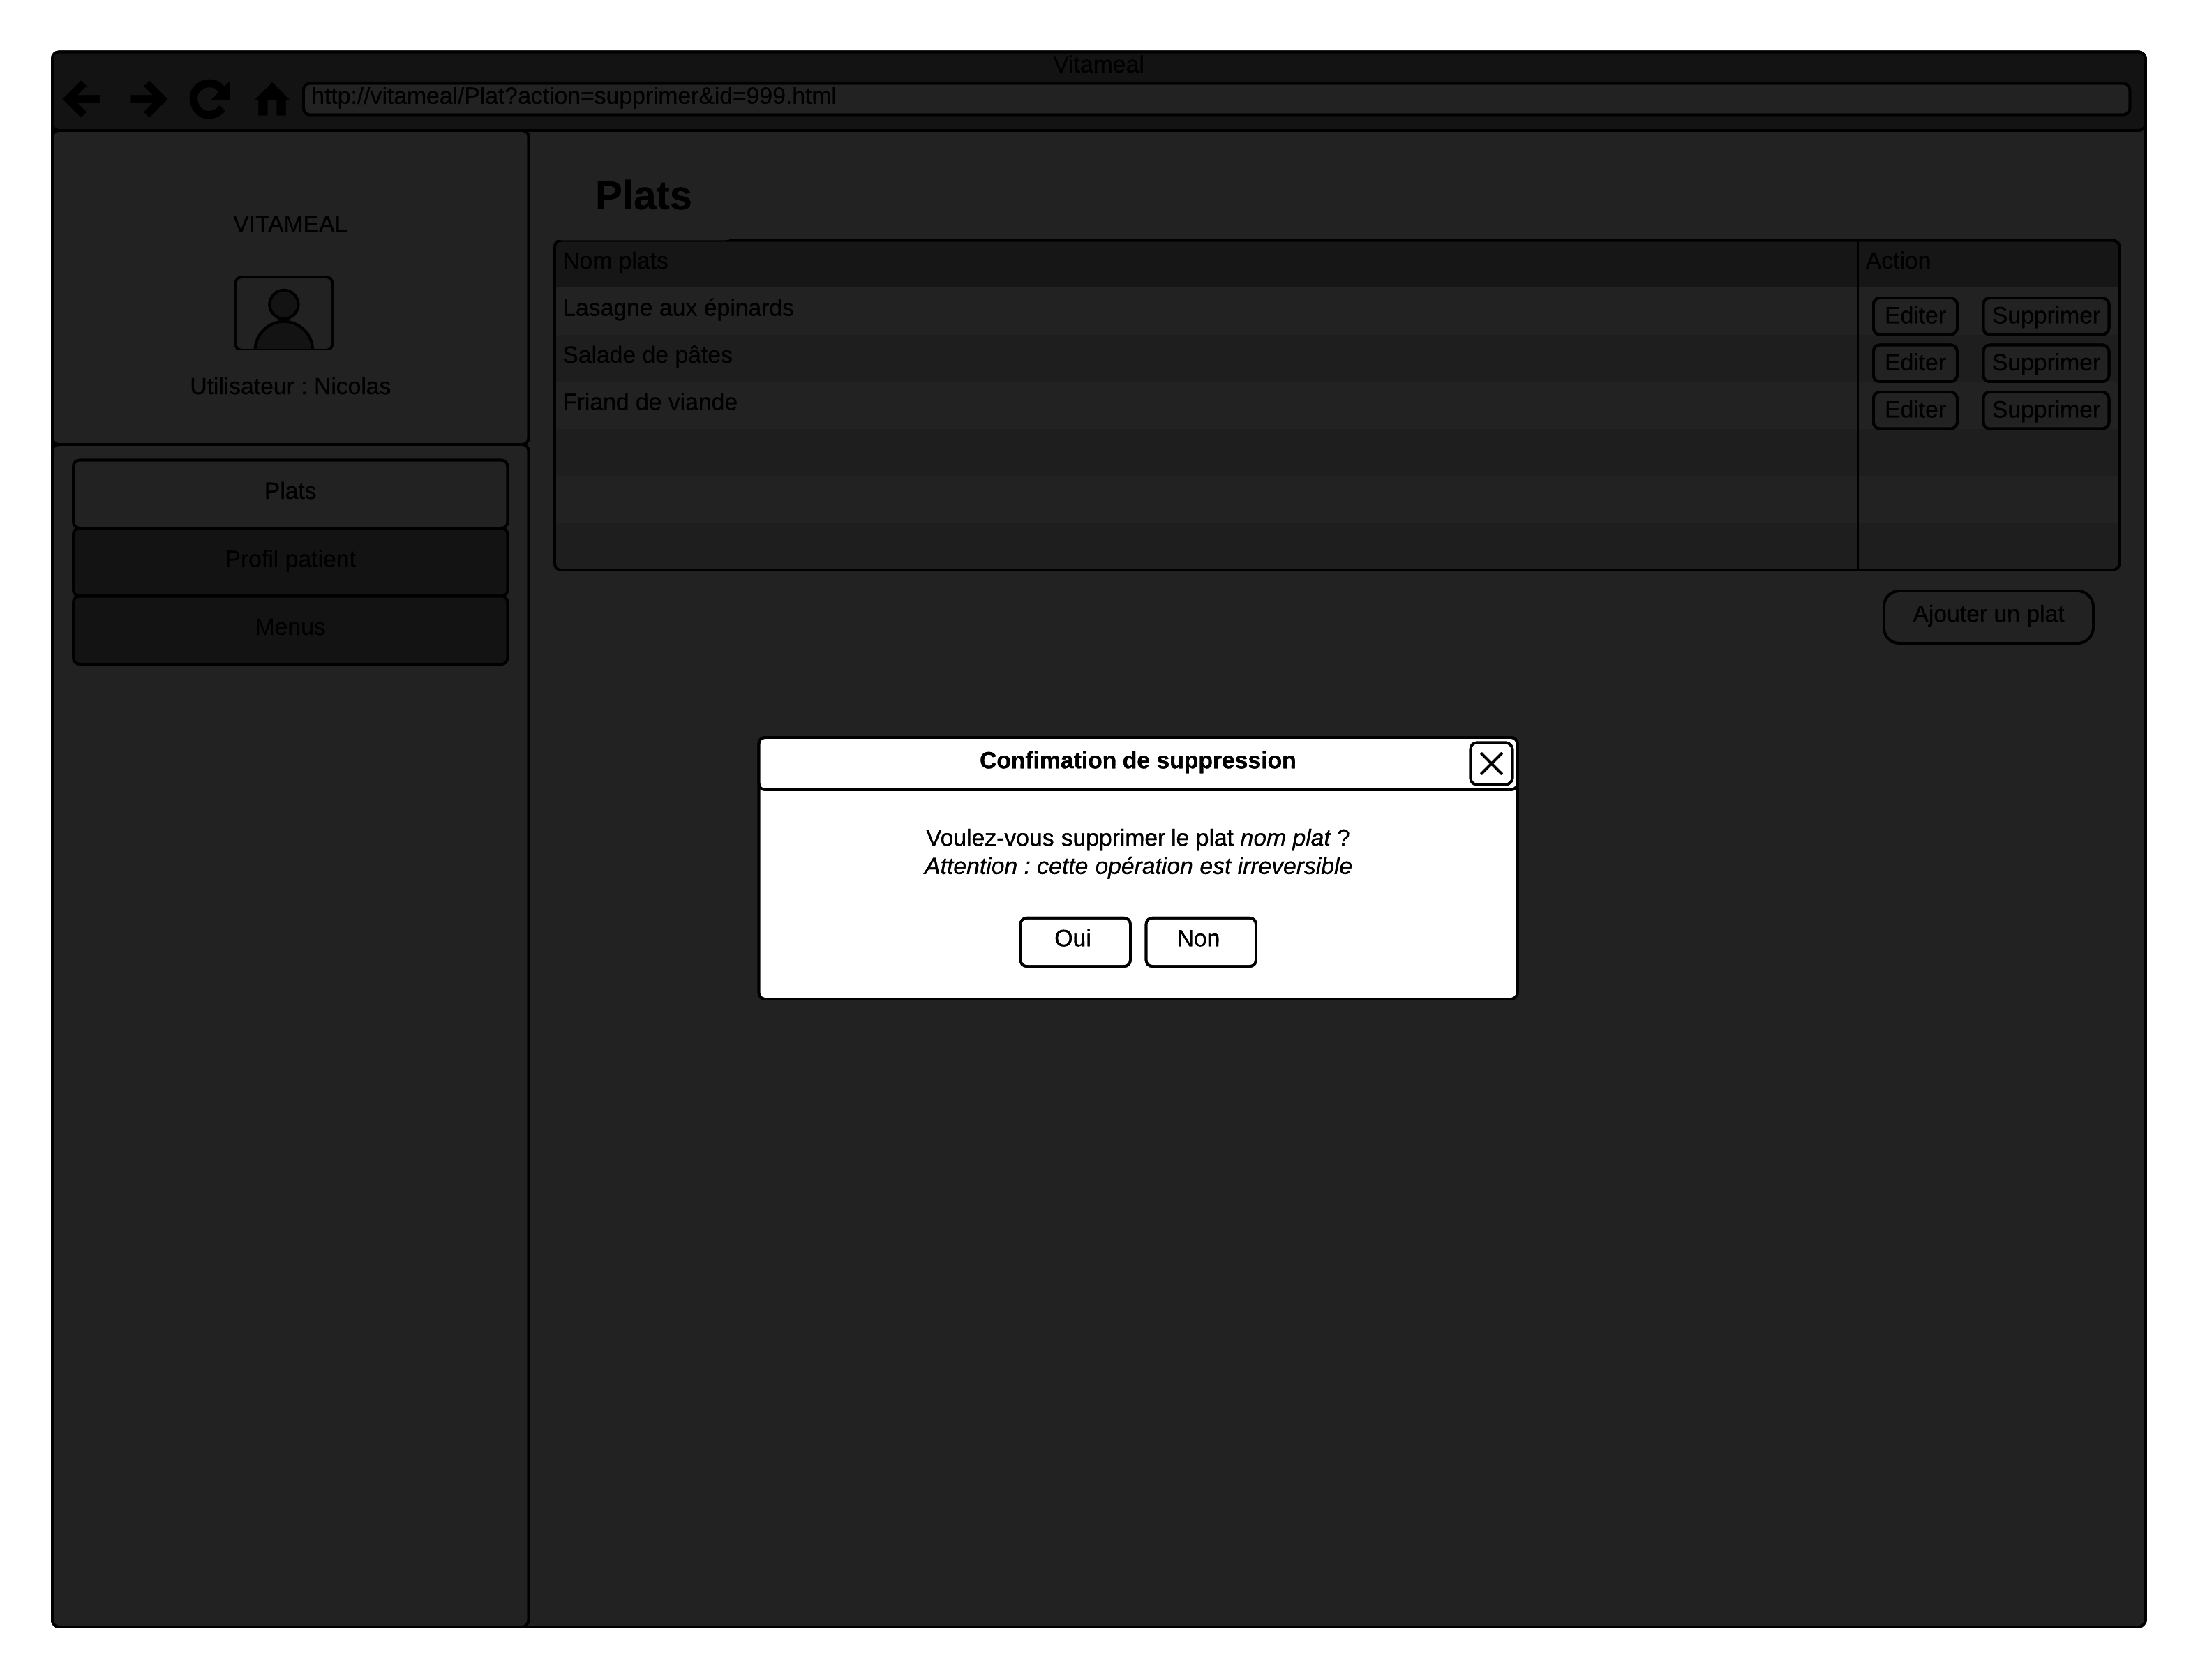
\includegraphics[scale=0.4]{../CasDUtilisations/CompositionPlat/maquette_MessageSupressionPlat.png}
\caption{Maquette de suppression d'un plat}
\label{MaquetteSuppressionPlat}
\end{figure}
\end{frame}

\begin{frame}[plain]{}
\begin{figure}
\centering
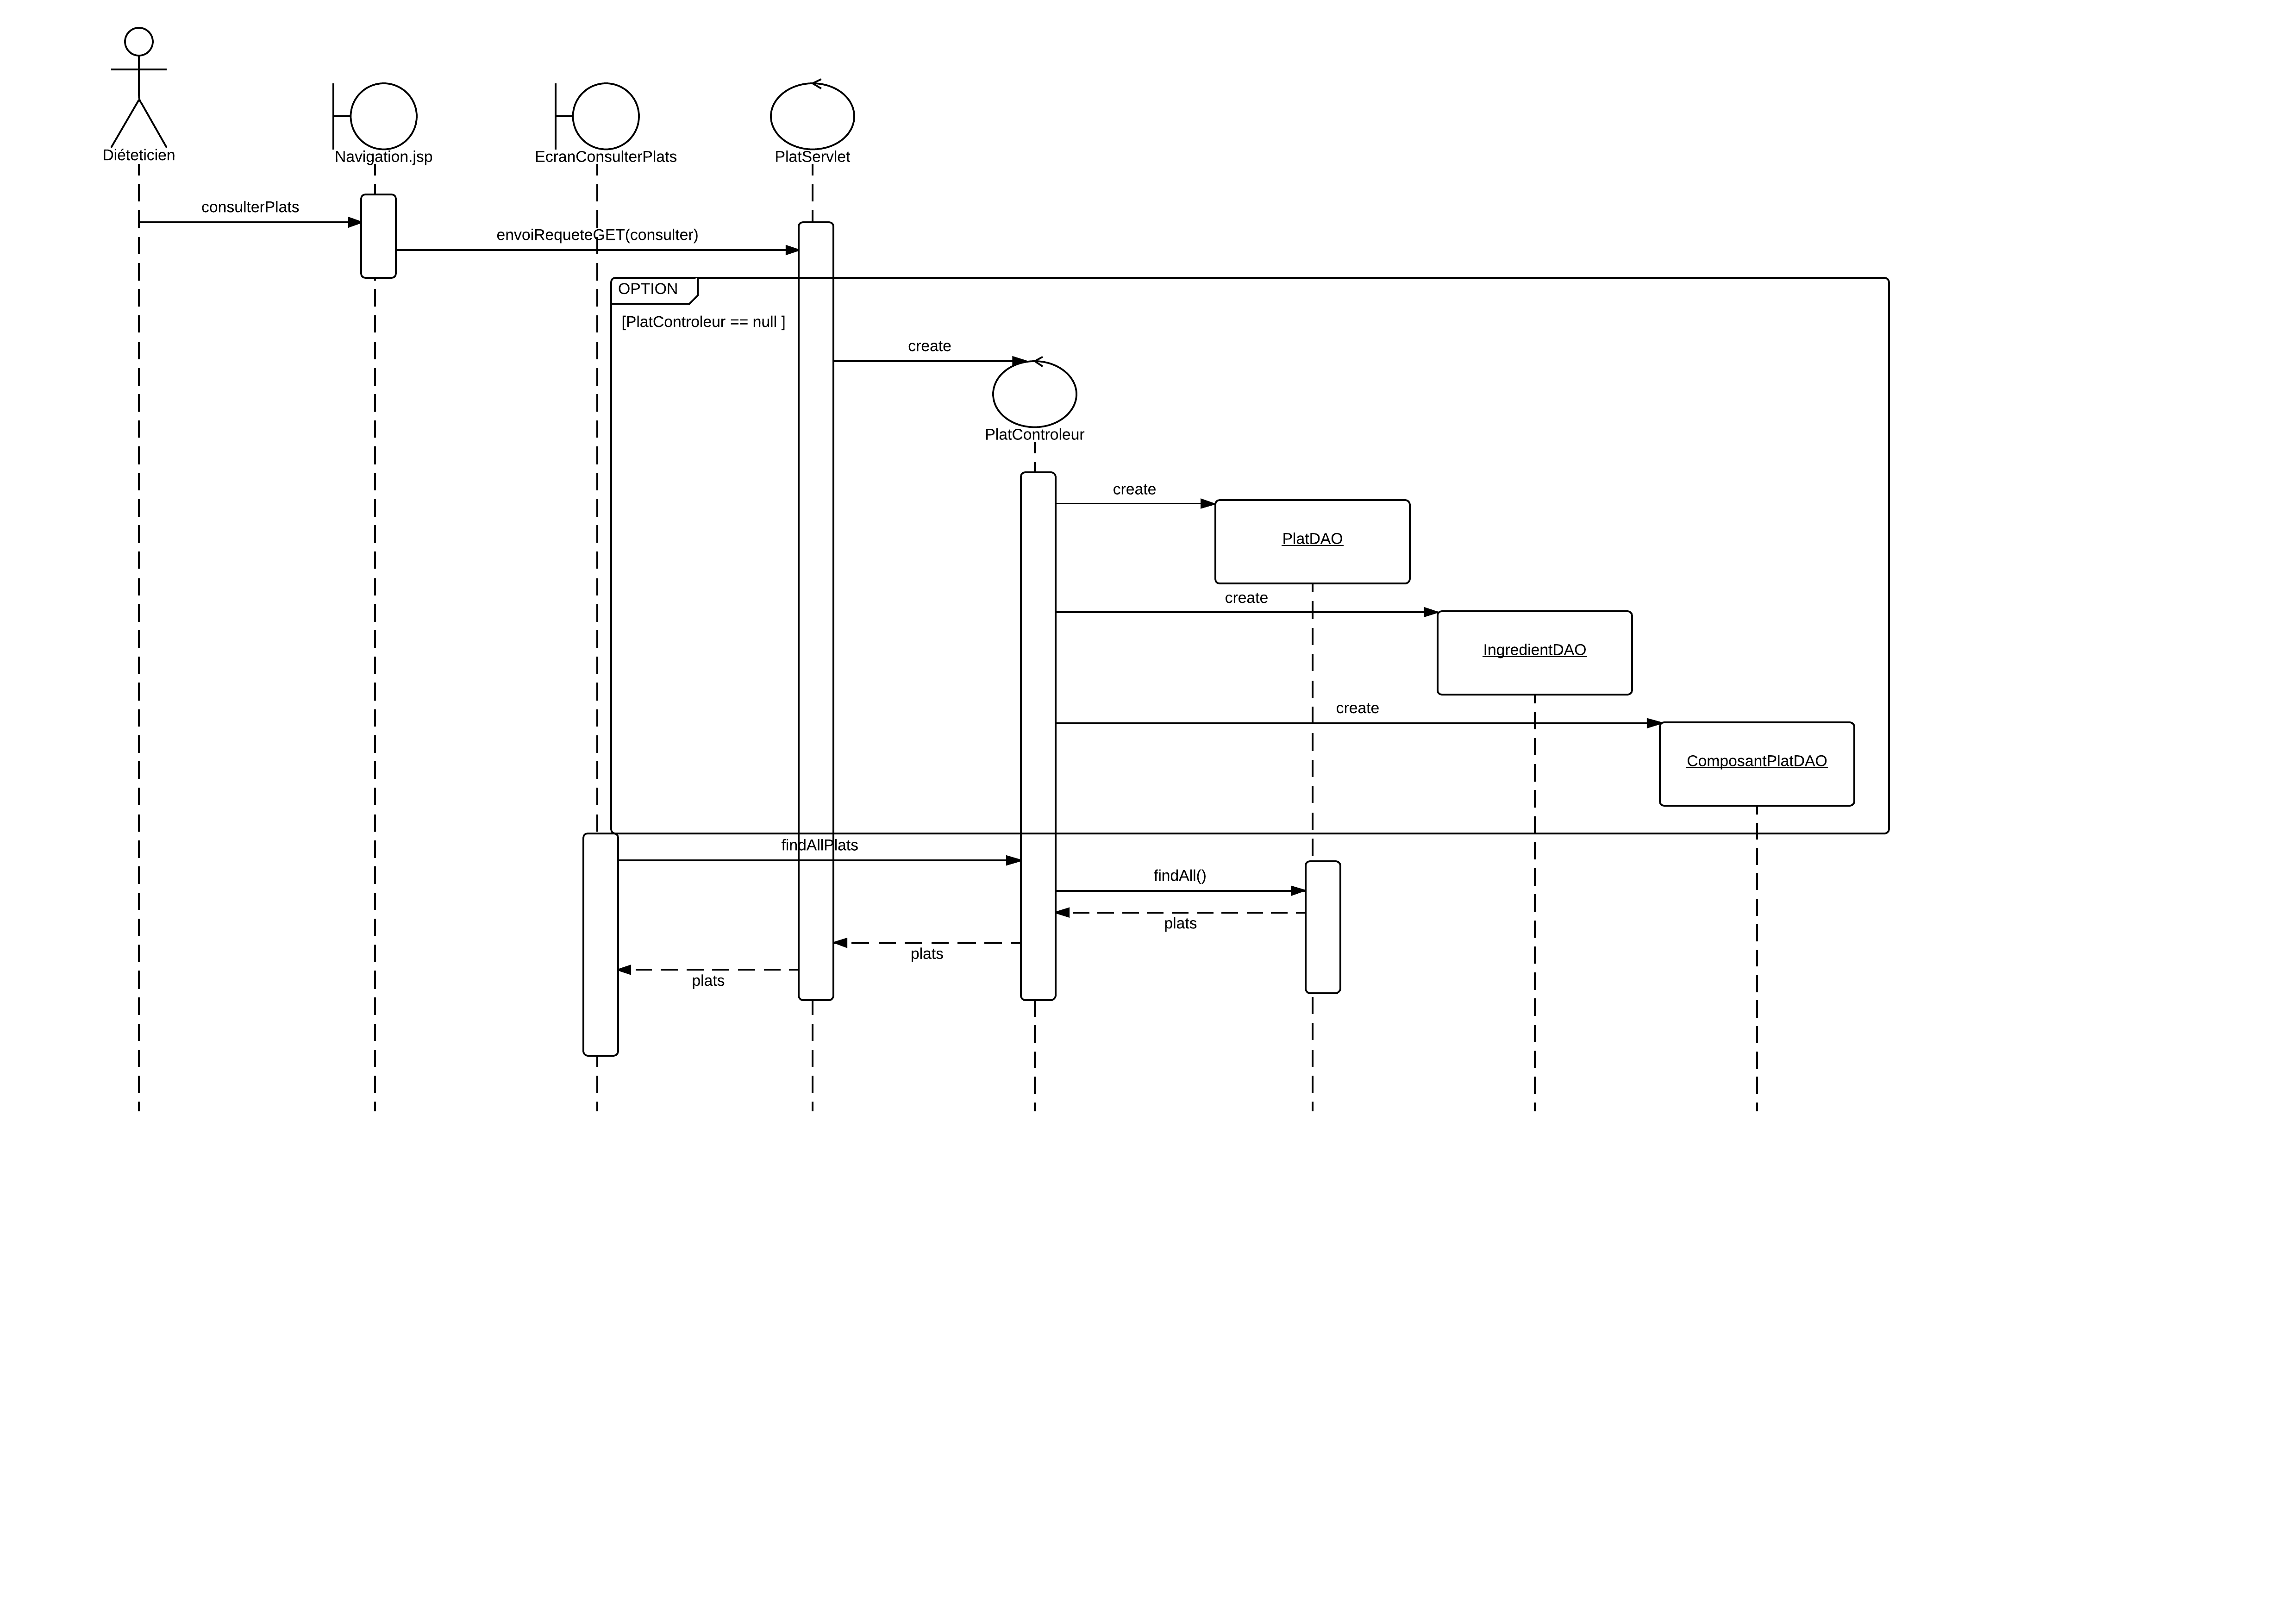
\includegraphics[scale=0.11]{../CasDUtilisations/CompositionPlat/sequence_InitialisationPlatControleur.png}
\end{figure}
\end{frame}

\begin{frame}[plain]{}
\begin{figure}
\centering
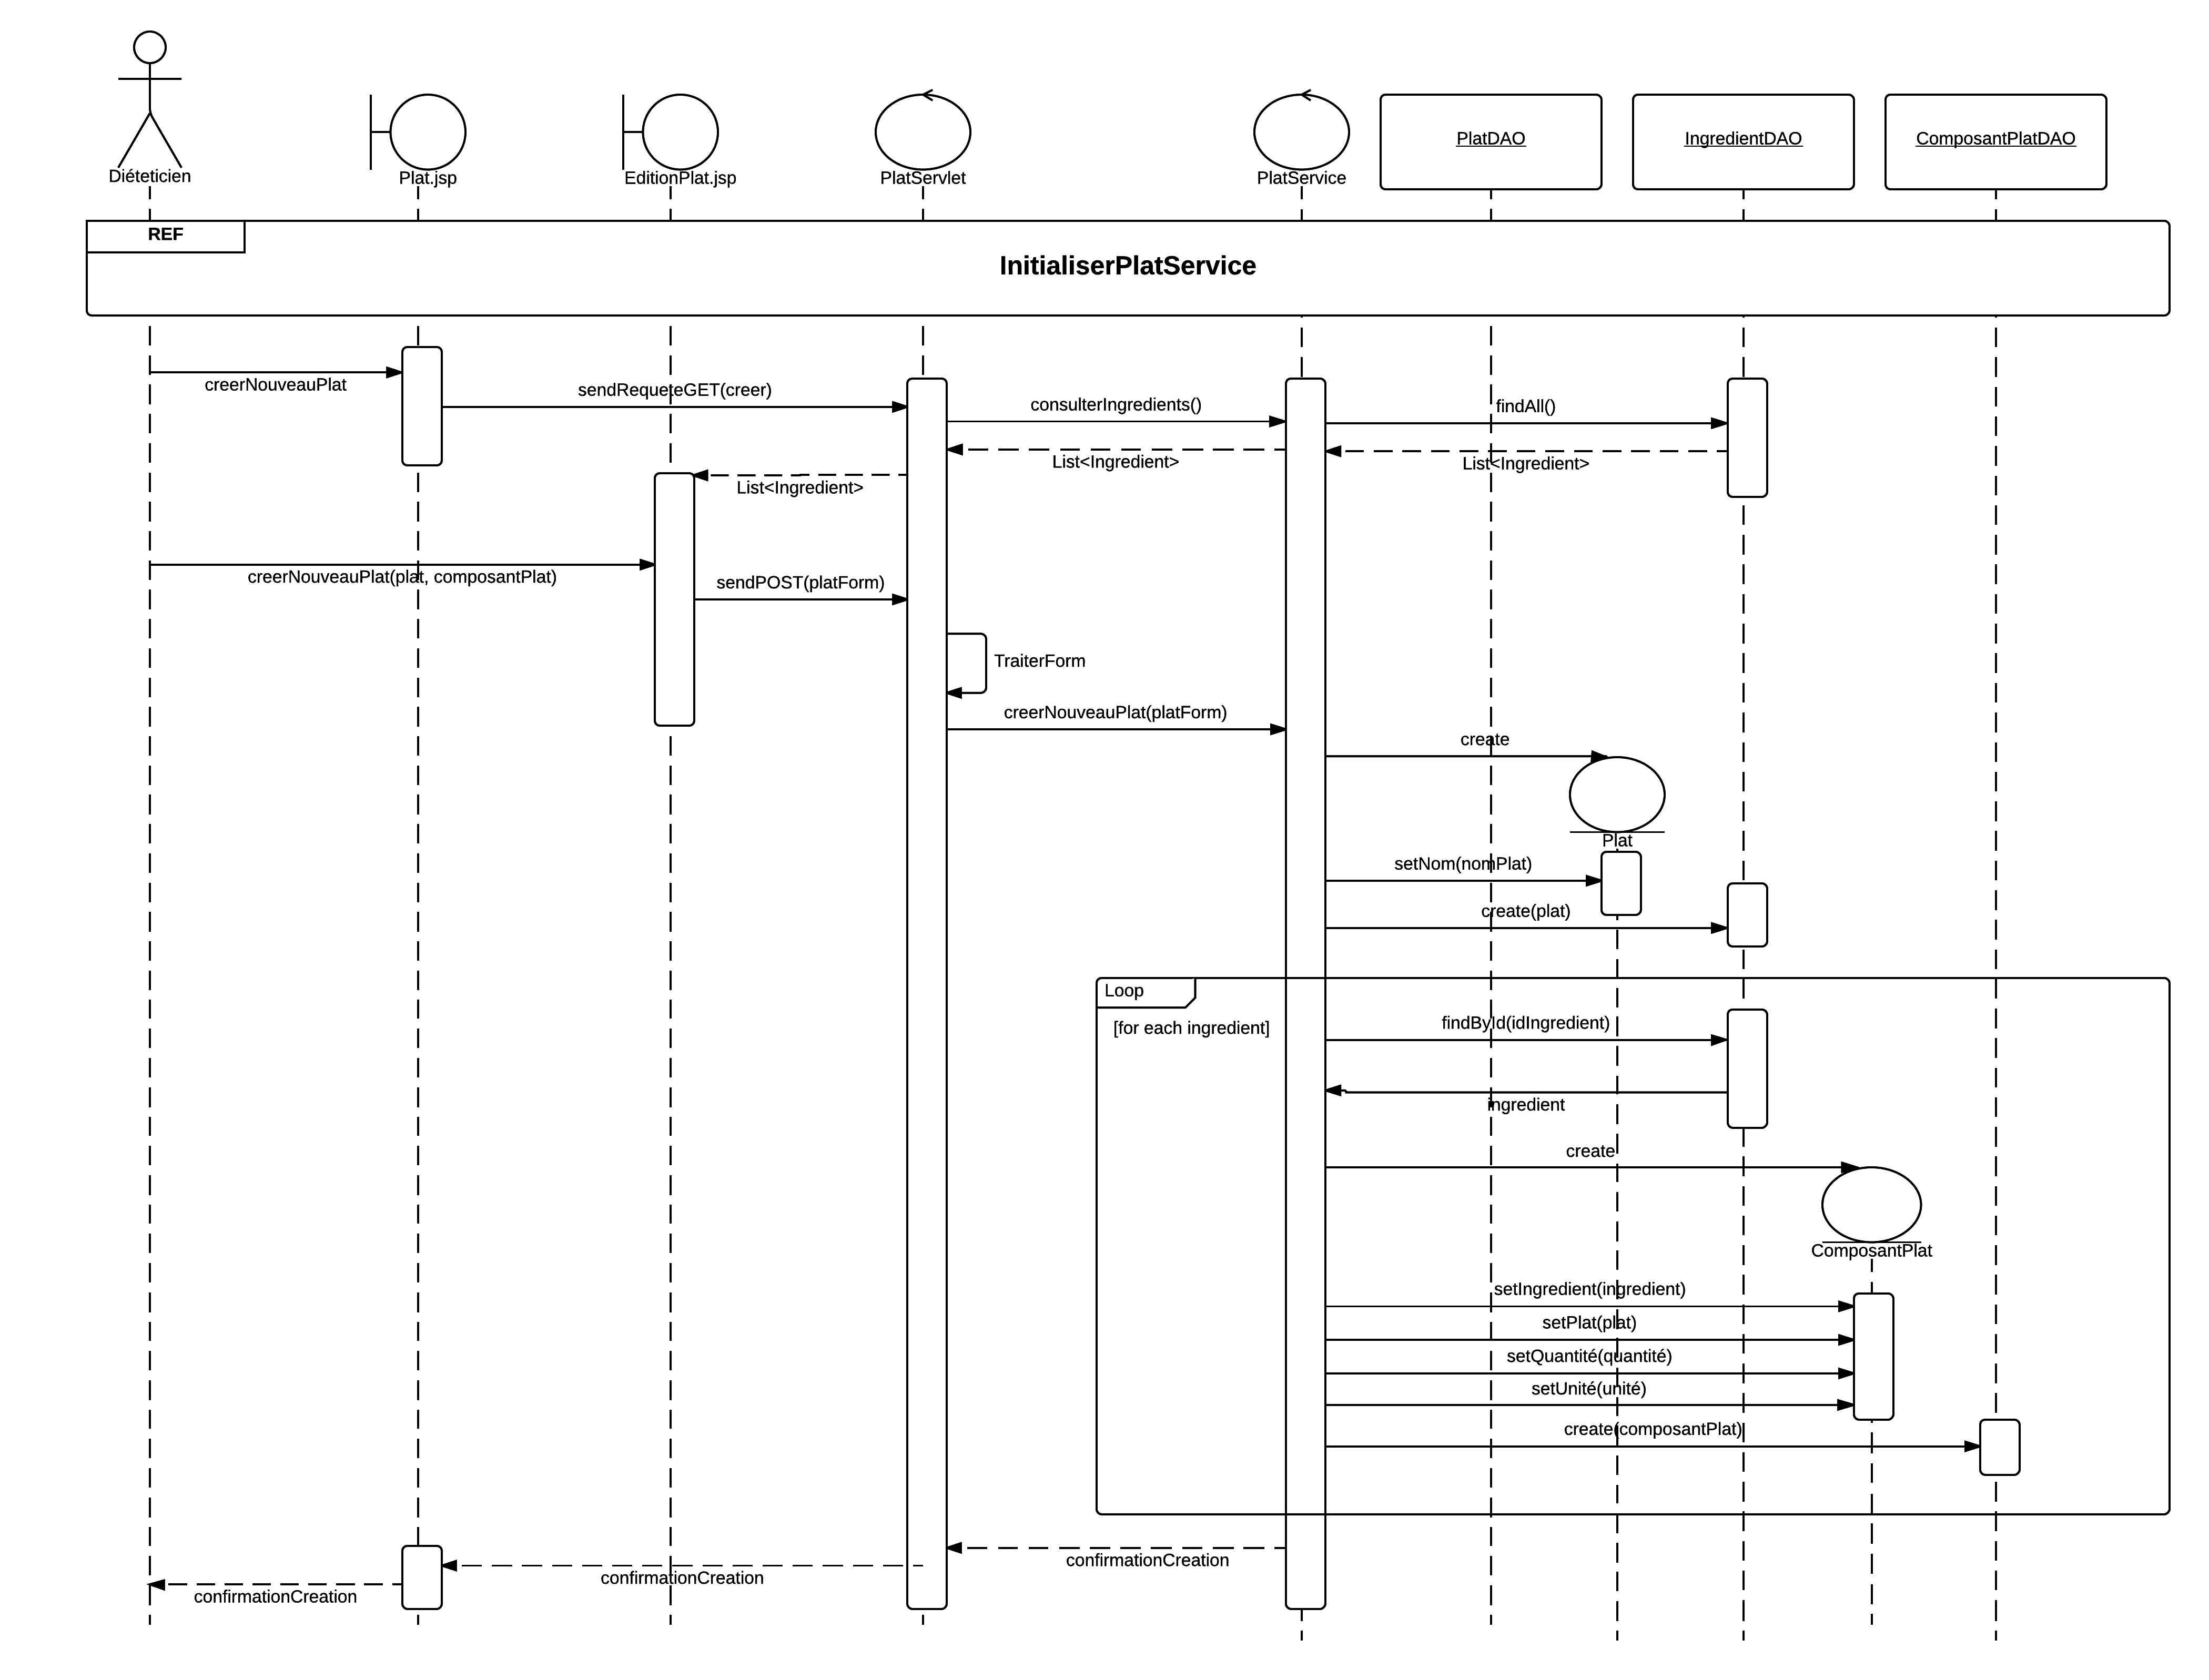
\includegraphics[scale=0.325]{../CasDUtilisations/CompositionPlat/sequence_CreerPlat.png}
\end{figure}
\end{frame}

\begin{frame}[plain]{}
\begin{figure}
\centering
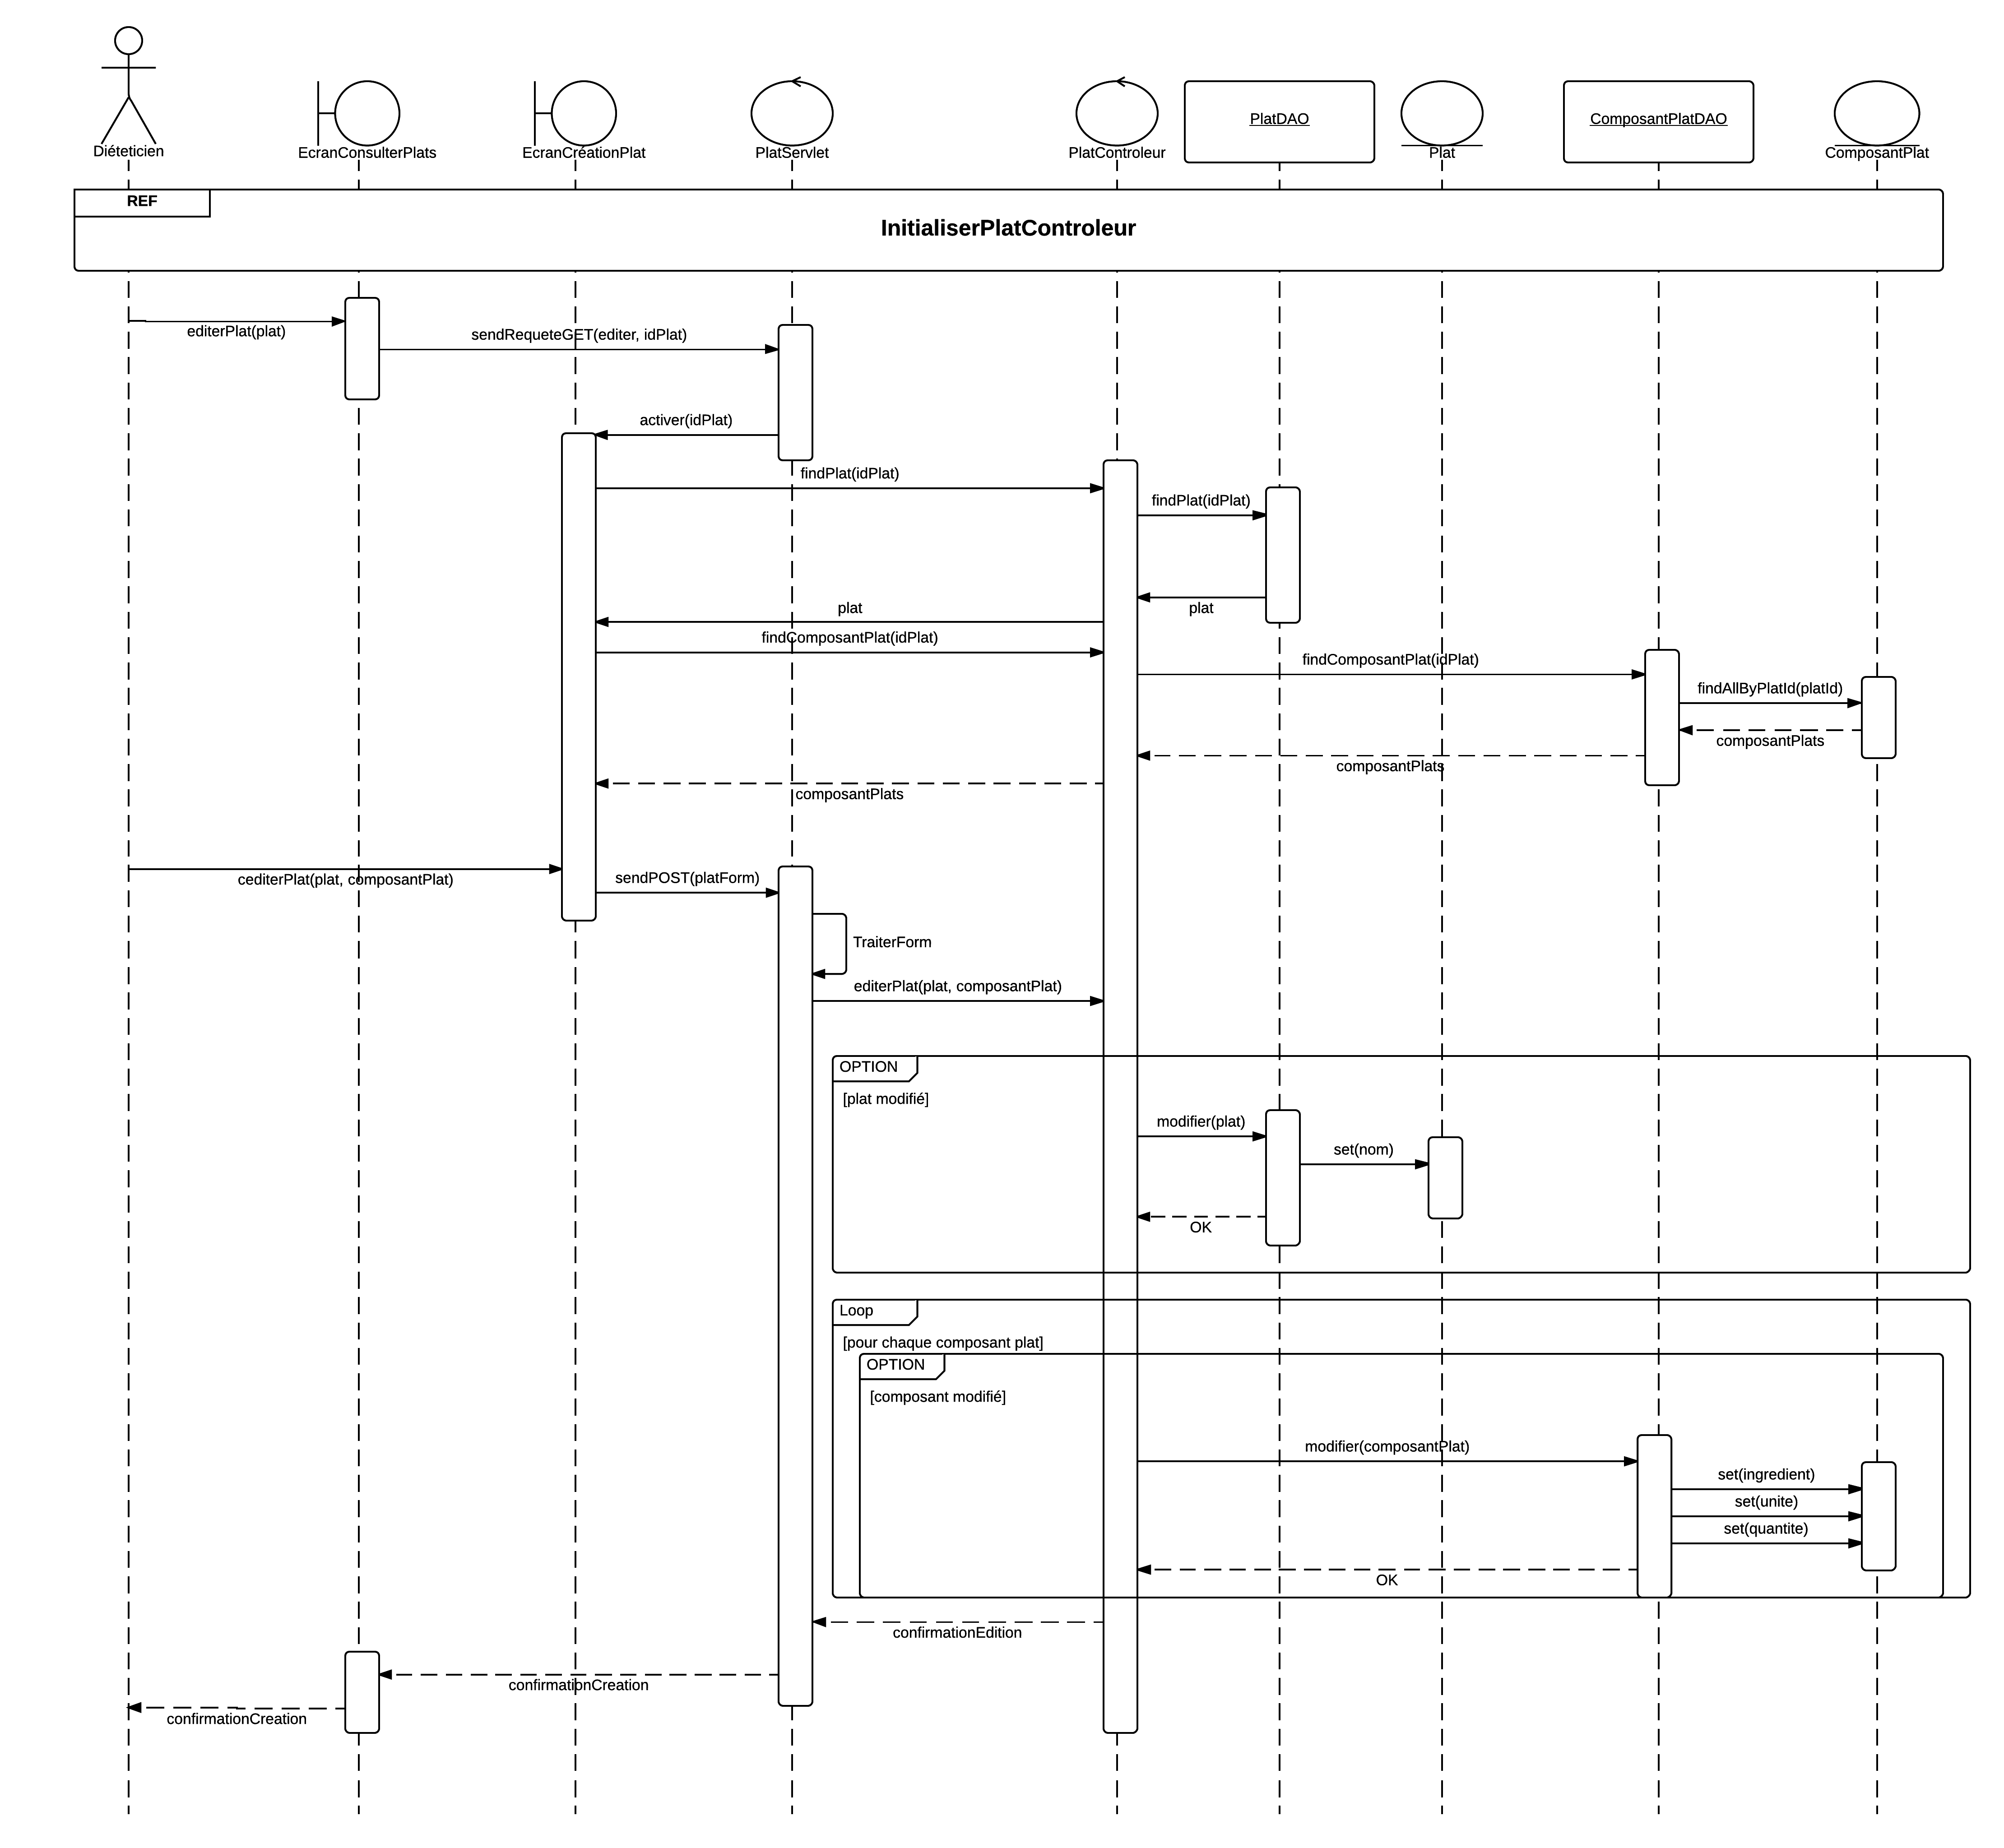
\includegraphics[scale=0.275]{../CasDUtilisations/CompositionPlat/sequence_EditerPlat.png}
\end{figure}
\end{frame}

\begin{frame}[plain]{}
\begin{figure}
\centering
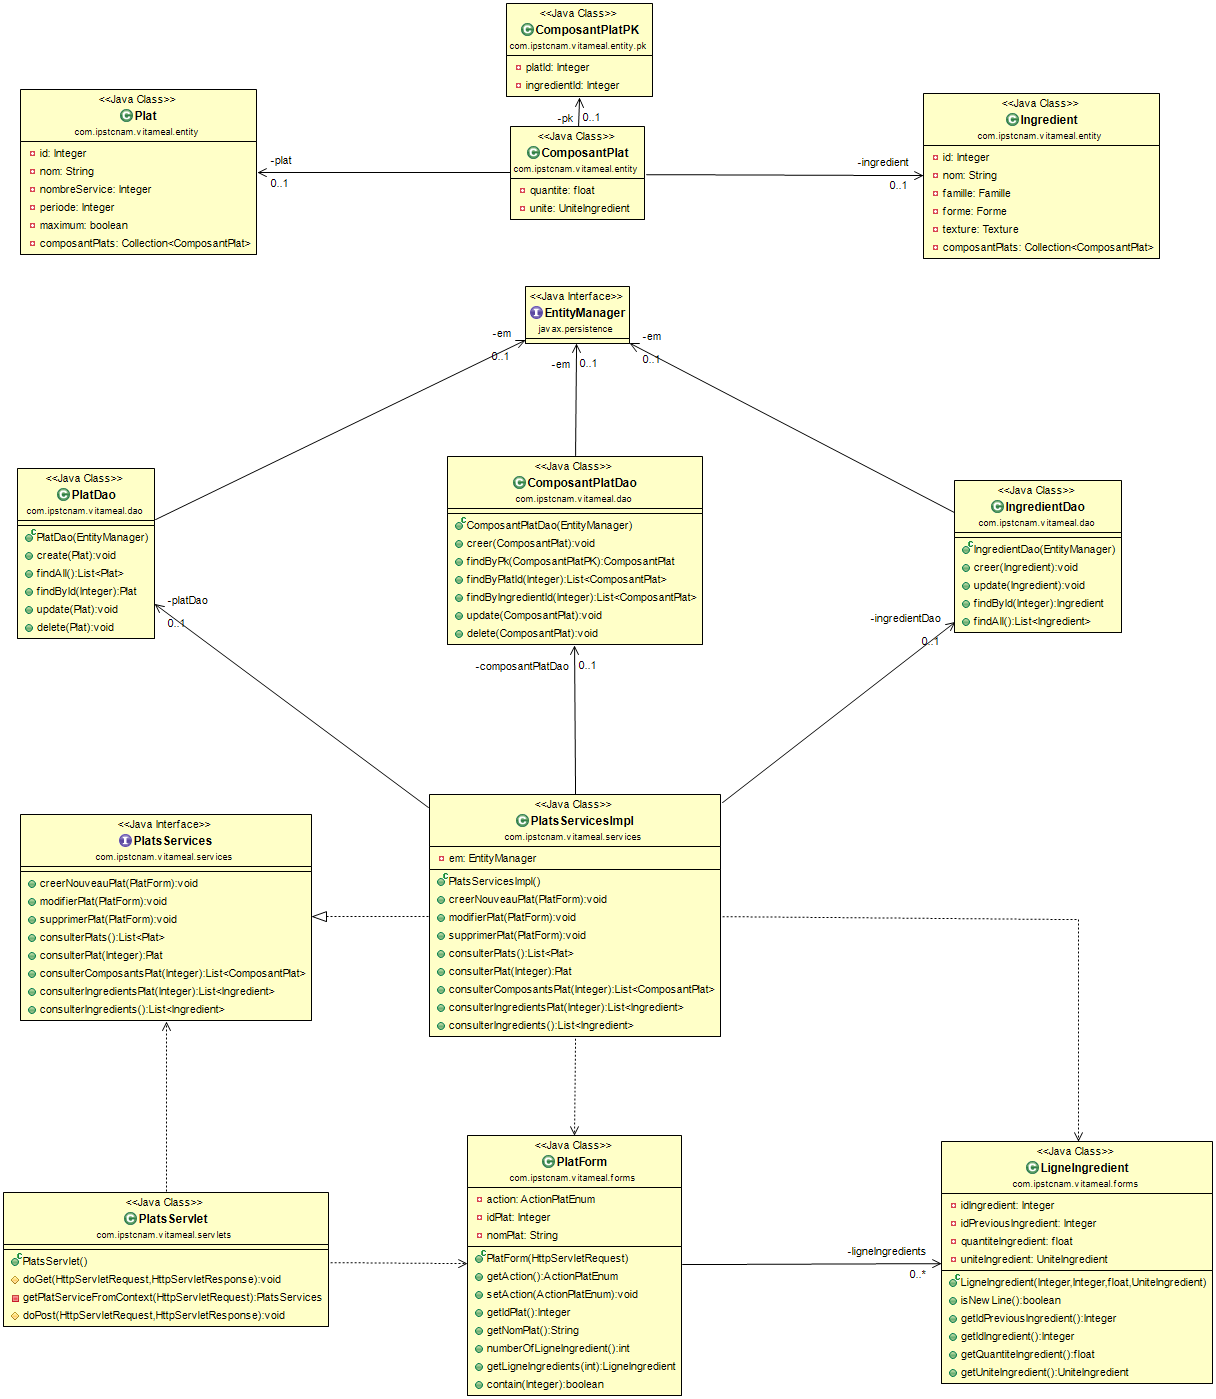
\includegraphics[scale=0.175]{../CasDUtilisations/CompositionPlat/classDiagram_ComposerPlat.png}
\end{figure}
\end{frame}

\subsection{Génération des menus}
\begin{frame}[plain]{}
%\frametitle{Génération des menus}
%%-*- coding: utf-8 -*-
\subsubsection{Élaboration des menus}
\begin{figure}
  \centering
      \includegraphics[width=1.00\textwidth]{../../CasDUtilisations/MenuGen/CasDUtilisation/MenuGen.png} %
\caption{Cas d'utilisation élaboration des menus}
\label{MenuGenCU}
\end{figure}

\begin{description}
\item[Nom:] Élaboration des menus (Figure \ref{MenuGenCU}).
\item[ID:] UC300
\item[Description:] Permet l'élaboration des menus.
\item[Auteur:] Jean-Félix BENITEZ.
\item[Date:] 15/06/2017
\item[Acteurs:] Diététiciens.
\item[Pré-Conditions:] Le diététicien s'est connecté au système.
\item[Scénario principal:] Figure \ref{MenuGenSeq}
  \begin{enumerate}
  \item Le diététicien sélectionne le groupe de patients pour lequel il veut générer les menus,
  \item \label{LanceElab}ensuite il lance l'élaboration des menus.
  \item L'élaboration automatique ce déroule en prenant en compte les grammages.
  \item Lorsque les menus sont élaborés, s'il estime l'élaboration correcte, il la valide.
  \item S'il estime l'élaboration incorrecte, il peut la rejeter, auquel cas il reviens à l'étape \ref{LanceElab}
  \item S'il estime l'élaboration incorrecte, il peut aussi la modifier manuellement.
  \end{enumerate}
\item[Scénario alternatif:] Aucun.
\item[Post-Conditions:] Les menus sont générés.
\end{description}

\begin{figure}
  \centering
      \includegraphics[width=1.00\textwidth]{../../CasDUtilisations/MenuGen/Sequence/ElaborationMenus.png} %
\caption{Séquence élaboration des menus}
\label{MenuGenSeq}
\end{figure}

\begin{figure}
\centering
\includegraphics[scale=.500]{../CasDUtilisations/MenuGen/CasDUtilisation/MenuGen.png}
\end{figure}
\end{frame}

\begin{frame}[plain]{}
\begin{figure}
\centering
\includegraphics[scale=0.080]{../CasDUtilisations/MenuGen/Sequence/ElaborationMenus.png}
\end{figure}
\end{frame}

\begin{frame}[plain]{}
\begin{figure}
\centering
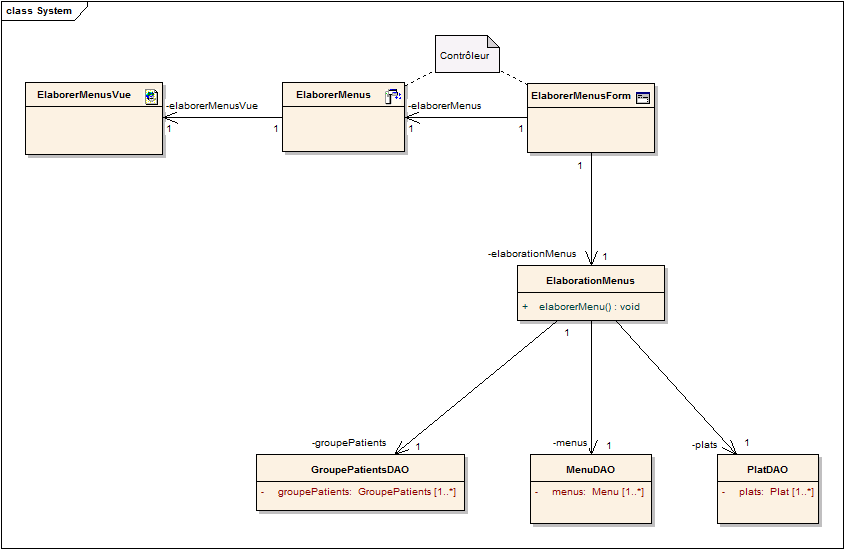
\includegraphics[scale=0.250]{../CasDUtilisations/MenuGen/Classes/EMC.png}
\end{figure}
\end{frame}

\subsection{Affichage des menus}
\begin{frame}
\frametitle{Affichage des menus}
\subsection{Diagramme afficher les menus
générés}\label{diagramme-afficher-les-menus-guxe9nuxe9ruxe9s}

\begin{figure}
\centering
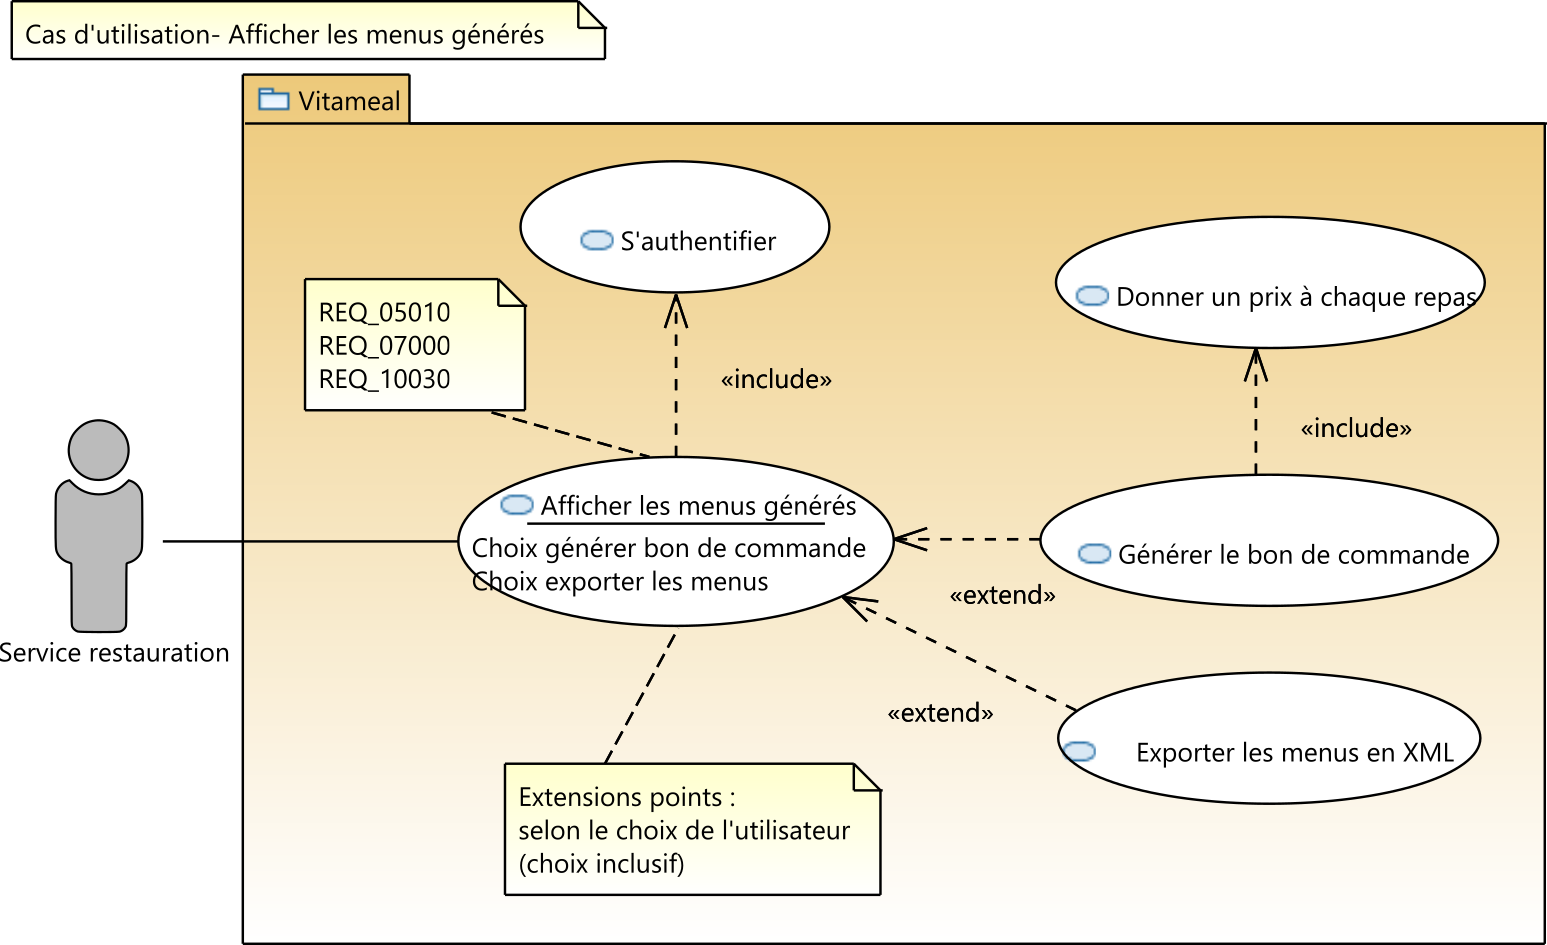
\includegraphics[width=0.85\textwidth]{../../CasDUtilisations/AfficherMenu/uc_afficher_menu.png}
\caption{Use case afficher les menus générés}
\end{figure}

\subsubsection{UC200 - Afficher les menus
générés}\label{uc200---afficher-les-menus-guxe9nuxe9ruxe9s}

\noindent\textbf{Nom :} Modifier un plat existant\\
\textbf{ID :} UC200\\
\textbf{Description :} Le service restauration souhaite pouvoir voir le
menu généré et selon son choix imprimer un bon\\
de commande et/ou exporter le menu sous un autre format.\\
\textbf{Auteur :} Nicolas SYMPHORIEN\\
\textbf{Dates(s) :} 08/05/2017\\
\textbf{Acteurs :} Le service restauration, par héritage, le diététicien
et le médecin\\
\textbf{Pré-condition :} L'utilisateur doit être identifié

\textbf{Scénario principal :}\\
1. Le système affiche un menu pour un groupe de patient donné 2.
L'utilisateur peut choisir de générer et voir le bon de commande associé
au menu affiché et l'utilisateur peut choisir de exporter le menu (pour
un usage par une tierce application)

\textbf{Scénario alternatif :}\\
1.a L'utilisateur peut changer de groupe de patient 1.b Le système
n'arrive pas à récupérer les menu générés 1.c Le système ne possède pas
de menu généré, il affiche un message d'information à l'utilisateur

\textbf{Post-Conditions:} Le menu est affiché. Un bon de commande est
produit. Un export est produit.

\subsubsection{UC201 - Générér le bon de
commande}\label{uc201---guxe9nuxe9ruxe9r-le-bon-de-commande}

\noindent\textbf{Nom :} Générer le bon de commande\\
\textbf{ID :} UC201\\
\textbf{Description :} Le service restauration souhaite pouvoir imprimer
un bon de commande du menu affiché\\
\textbf{Auteur :} Nicolas SYMPHORIEN\\
\textbf{Dates(s) :} 08/05/2017\\
\textbf{Acteurs :} Le service restauration, par héritage, le diététicien
et le médecin\\
\textbf{Pré-condition :} L'utilisateur doit être identifié

\textbf{Scénario principal :}\\
1. Le système propose la génération du menu si le prix de chaque plat a
été renseigné

\textbf{Scénario alternatif :}\\
1. a. Le prix de chaque plat n'a pas été renseigné

\textbf{Post-Conditions:} Le bon de commande et généré et affiché.

\subsubsection{UC202 - Donner un prix à chaque
repas}\label{uc202---donner-un-prix-uxe0-chaque-repas}

\noindent\textbf{Nom :} Donner un prix à chaque repas\\
\textbf{ID :} UC202\\
\textbf{Description :} Le service restauration souhaite pouvoir donnée
le pris de chaque plat composant un menu\\
\textbf{Auteur :} Nicolas SYMPHORIEN\\
\textbf{Dates(s) :} 08/05/2017\\
\textbf{Acteurs :} Le service restauration, par héritage, le diététicien
et le médecin\\
\textbf{Pré-condition :} L'utilisateur doit être identifié

\textbf{Scénario principal :}\\
1. Le système propose de renseigner le prix du plat

\textbf{Scénario alternatif :} aucun

\textbf{Post-Conditions:} Le prix du plat est renseigné

\subsubsection{UC203 - Exporter le menu affiché au format
XML}\label{uc203---exporter-le-menu-affichuxe9-au-format-xml}

\noindent\textbf{Nom :} Exporter le menu affiché au format XML\\
\textbf{ID :} UC203\\
\textbf{Description :} Le service restauration souhaite pouvoir exporté
le menu affiché pour un usage dans une tierce application (comme le site
internet de l'hopital par exemple)\\
\textbf{Auteur :} Nicolas SYMPHORIEN\\
\textbf{Dates(s) :} 08/05/2017\\
\textbf{Acteurs :} Le service restauration, par héritage, le diététicien
et le médecin\\
\textbf{Pré-condition :} L'utilisateur doit être identifié

\textbf{Scénario principal :}\\
1. Le système exporte le menu affiché en XML

\textbf{Scénario alternatif :} échec de l'export

\textbf{Post-Conditions:} Le menu est exportée au format XML

\end{frame}

\section{Modèle du domaine}
\begin{frame}[plain]{}
\begin{figure}
\centering
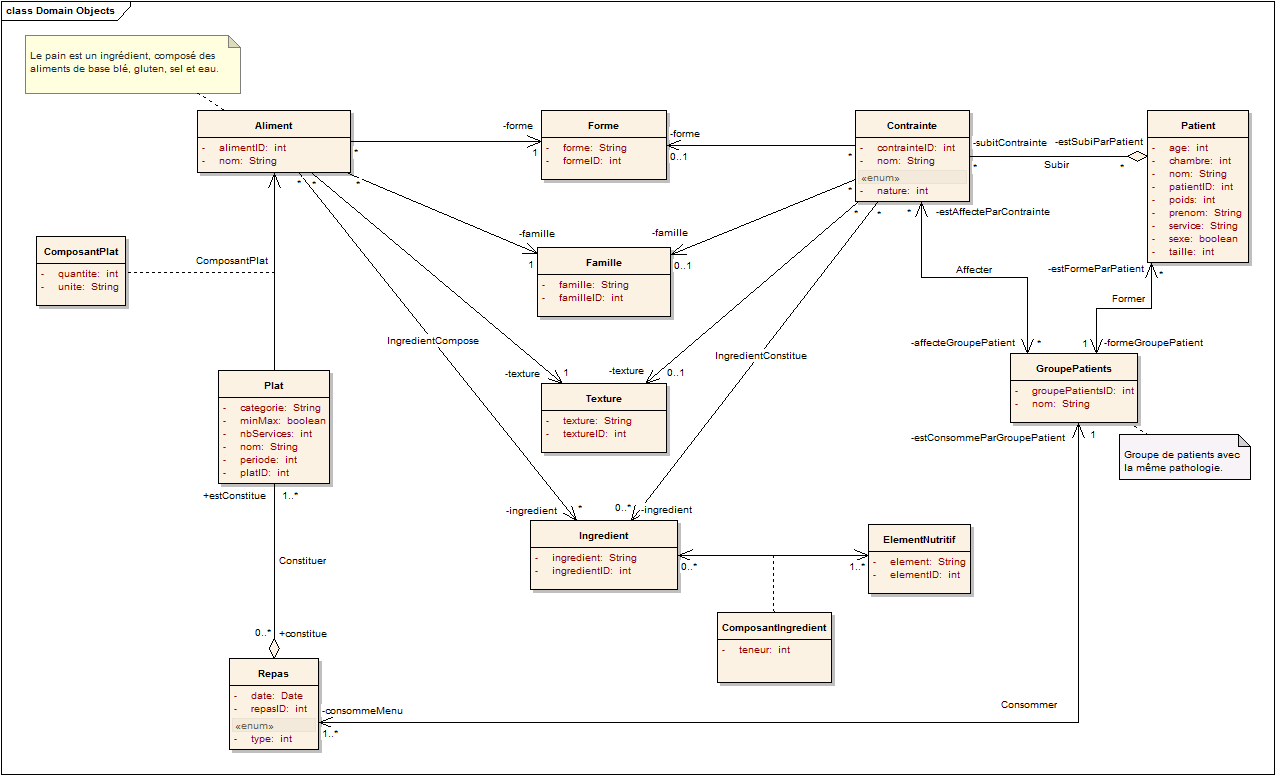
\includegraphics[scale=0.140]{../ModeleDuDomaine/ModeleDuDomaine.png}
\end{figure}
\end{frame}

\section{Planning}
\begin{frame}[label=planning]
\frametitle{Planning}
\begin{figure}[H]
\textbf{G}antt
\label{Gantt}
  \centering
      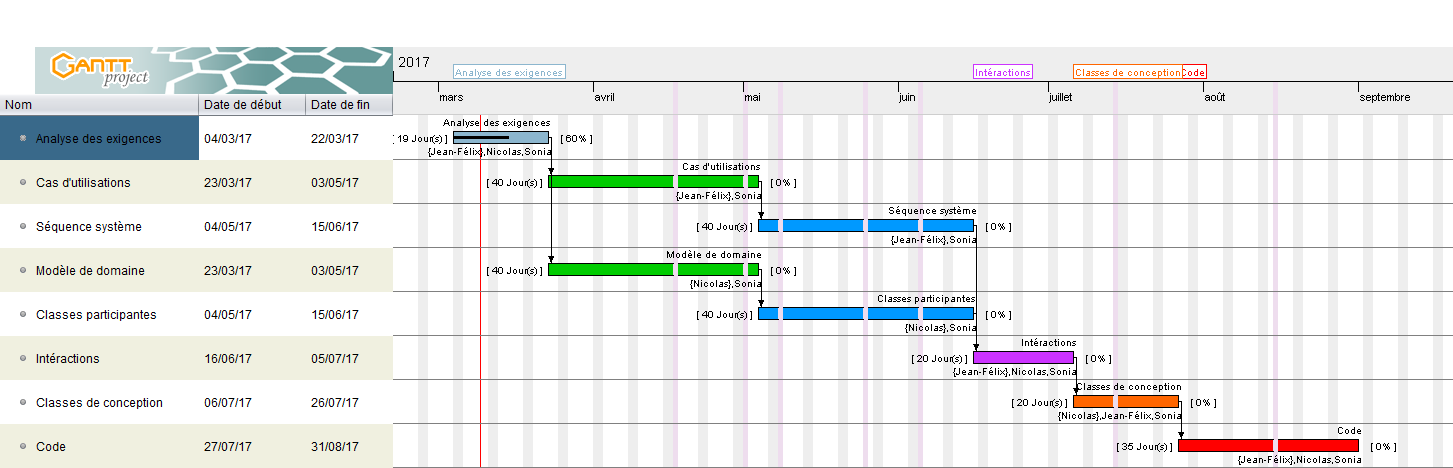
\includegraphics[width=0.95\textwidth]{Vitameal_gantt.png} %
%\caption{Gantt}
\end{figure}

\begin{figure}[H]
\textbf{P}rogram \textbf{E}valuation and \textbf{R}eview \textbf{T}echnique
\label{PERT}
  \centering
      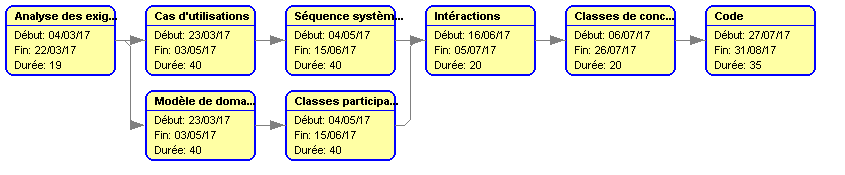
\includegraphics[width=0.8\textwidth]{Vitameal_pert.png} %
%\caption{PERT}
\end{figure}
\end{frame}

\section{Usine logicielle}
\begin{frame}[label=schemaFonctionnement]
  \frametitle{Usine logicielle - Schéma de fonctionnement}
\begin{figure}[H]
\label{schema}
  \centering
      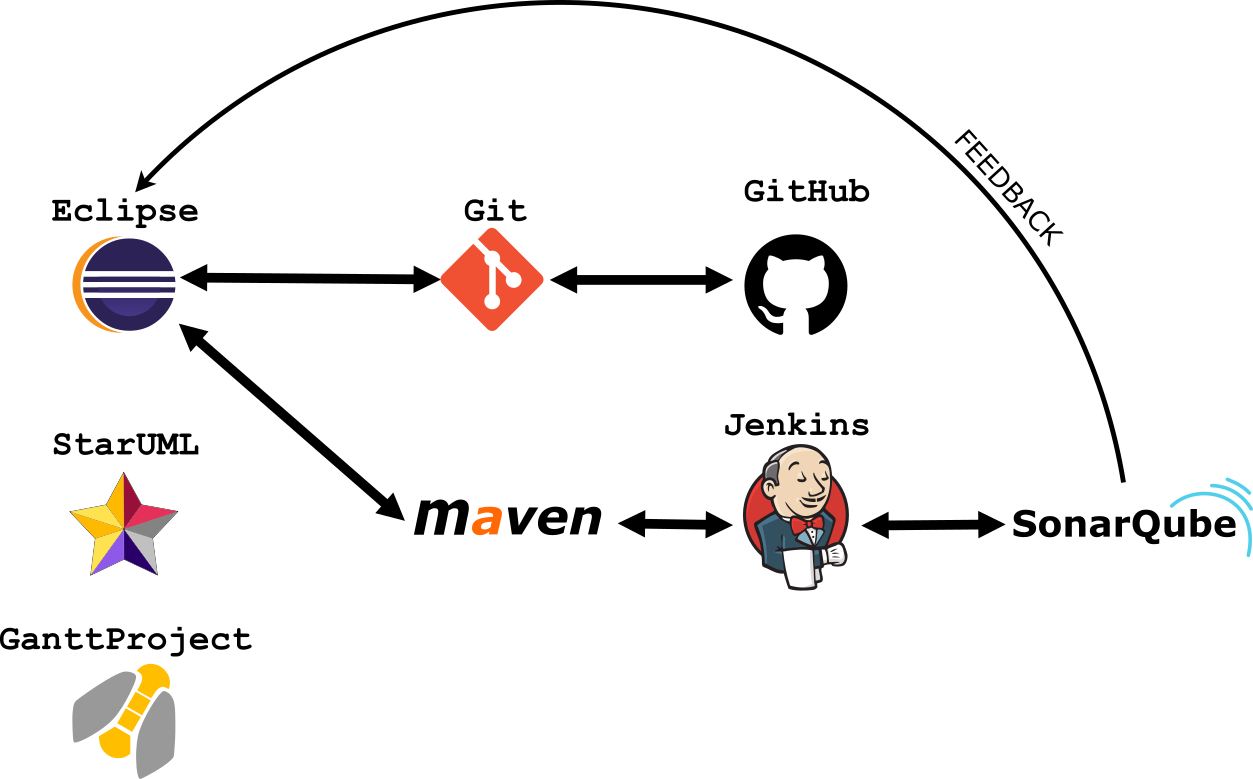
\includegraphics[width=1.0\textwidth]{usine_vitameal.png} %
%\caption{Schéma}
\end{figure}
\end{frame}

\section{Architecture générale}

\begin{frame}[label=Architecture 3-tiers]
  \frametitle{Architecture 3-tiers}
\begin{figure}[H]
\label{schema}
  \centering
      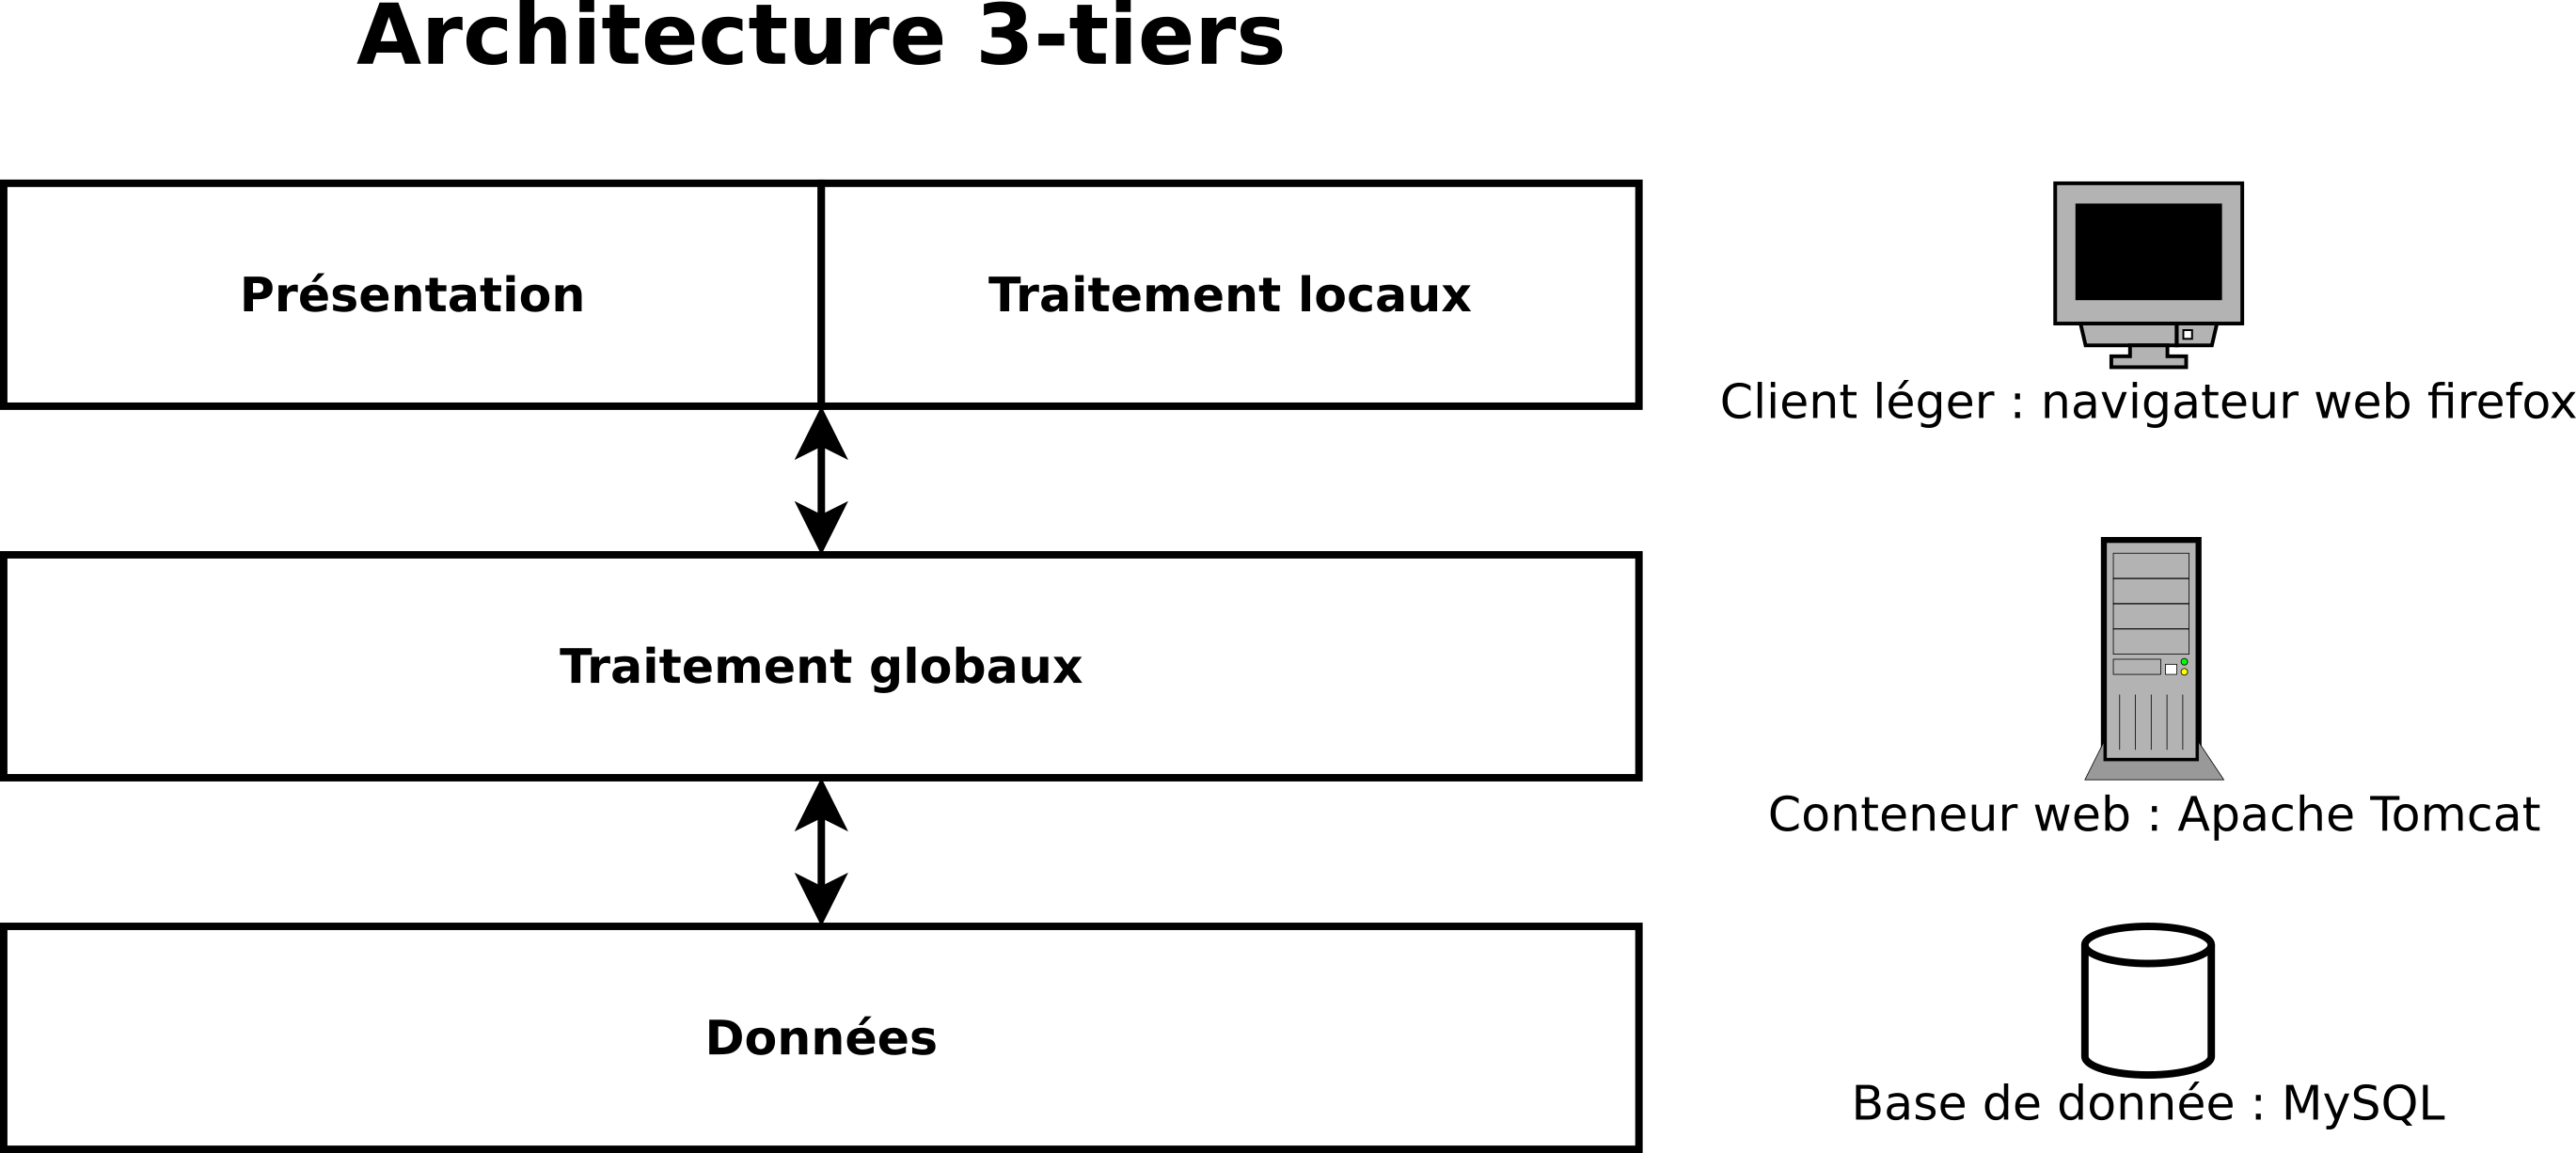
\includegraphics[width=1\textwidth]{architectureVitameal_3tiers.png} %
%\caption{Schéma}
\end{figure}
\end{frame}

\begin{frame}[label=Détails de l'architecture]
  \frametitle{Détails de l'architecture}
\begin{figure}[H]
\label{schema}
  \centering
      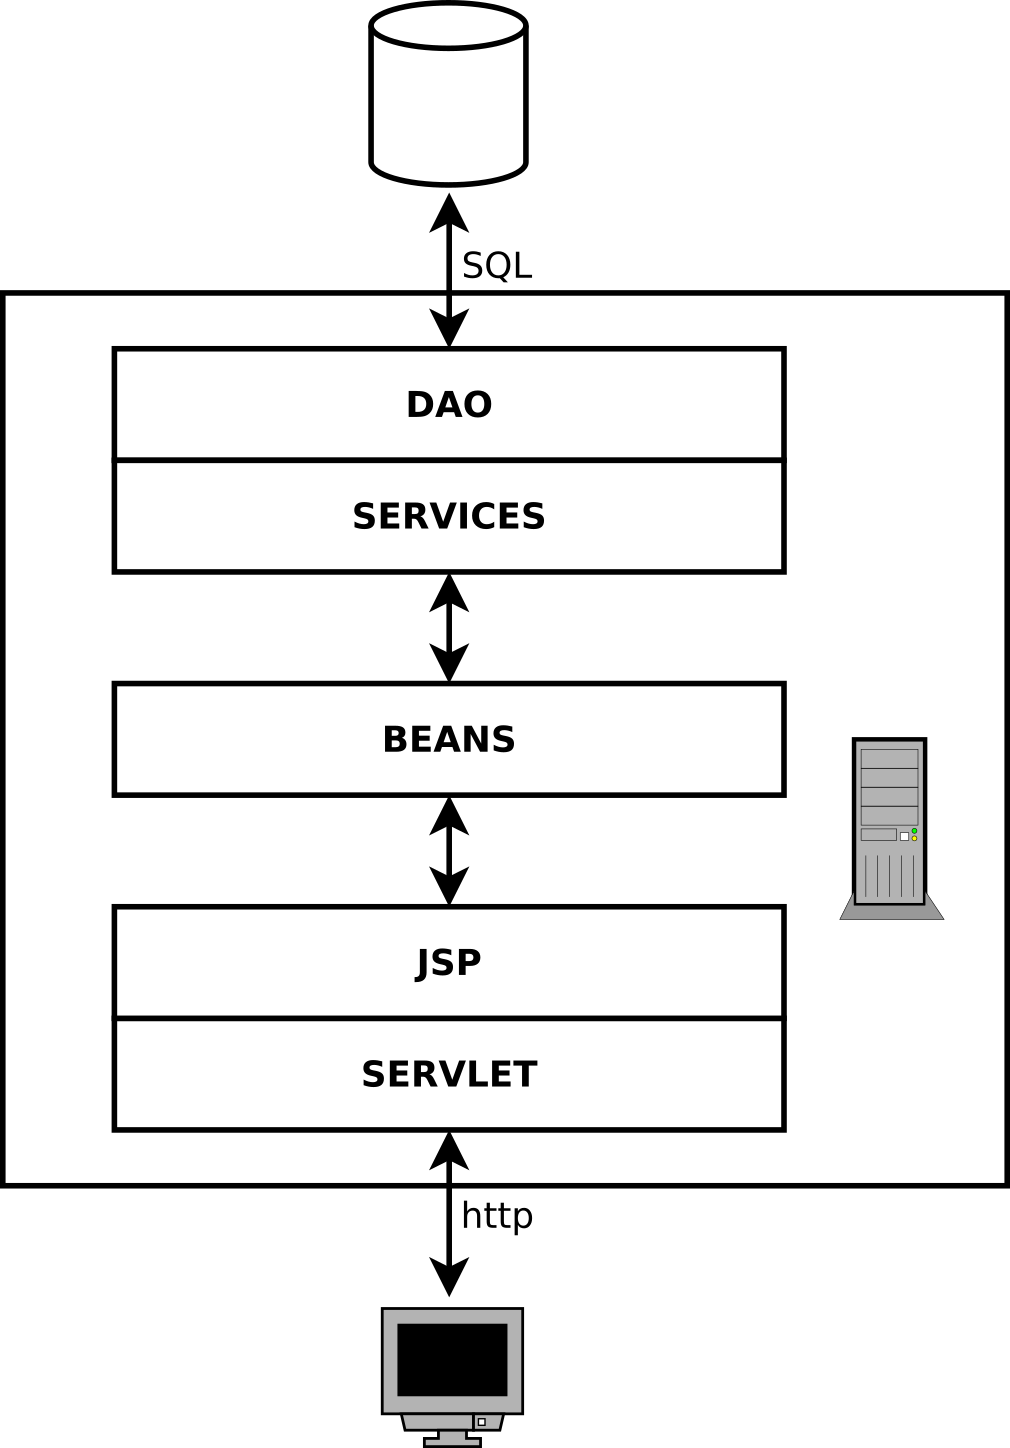
\includegraphics[width=0.35\textwidth]{architectureVitameal_details.png} %
%\caption{Schéma}
\end{figure}
\end{frame}

\end{document}
